% This is samplepaper.tex, a sample chapter demonstrating the
% LLNCS macro package for Springer Computer Science proceedings;
% Version 2.20 of 2017/10/04
%
\documentclass[runningheads]{llncs}
%
\usepackage{amsmath}
\usepackage{amssymb}
\usepackage{booktabs} % For pretty tables
\usepackage[labelfont=bf,font=scriptsize]{caption}
\usepackage[font=scriptsize]{subcaption}
\usepackage{graphicx}
\usepackage{pgfplots}
\usepackage[all]{nowidow}
\usepackage{multirow}
\usepackage{xcolor}

\usepackage[utf8]{inputenc}
\usepackage{tikz}
\usetikzlibrary{er,positioning,bayesnet}
\usepackage{multicol}
\usepackage{algpseudocode,algorithm,algorithmicx}
\usepackage{hyperref}
\usepackage[inline]{enumitem} % Horizontal lists
\newcommand{\indentitem}{\setlength\itemindent{20pt}}

\graphicspath{{latex/}}
\newcommand{\card}[1]{\left\vert{#1}\right\vert}
\newcommand*\Let[2]{\State #1 $\gets$ #2}
\newcommand\qfrac[3][1pt]{\frac{%
		\ThisStyle{\addstackgap[#1]{\SavedStyle#2}}}{%
		\ThisStyle{\addstackgap[#1]{\SavedStyle#3}}%
}}


\newcommand{\F}{\ensuremath{\mathbb{F}}}
\newcommand{\B}{\ensuremath{\mathbb{B}}}
\newcommand{\LL}{\ensuremath{\mathbb{L}}}
\newcommand{\Me}{\ensuremath{\mathbb{M}_e^{\text{eff}}}}
\newcommand{\D}{\ensuremath{\text{D}}}
\renewcommand{\d}{\ensuremath{\text{d}}}
\pgfplotsset{compat=1.14}

\renewcommand{\topfraction}{0.85}
\renewcommand{\bottomfraction}{0.85}
\renewcommand{\textfraction}{0.15}
\renewcommand{\floatpagefraction}{0.8}
\renewcommand{\textfraction}{0.1}
\setlength{\floatsep}{3pt plus 1pt minus 1pt}
\setlength{\textfloatsep}{3pt plus 1pt minus 1pt}
\setlength{\intextsep}{3pt plus 1pt minus 1pt}
\setlength{\abovecaptionskip}{2pt plus 1pt minus 1pt}


\begin{document}
%
\title{A thermodynamically consistent poro-visco-elastic model of the Extracellular Matrix}
%
\titlerunning{Mechanical Properties of ECM}
% If the paper title is too long for the running head, you can set
% an abbreviated paper title here
%
\author{Giulia Laura Celora}
%
%\authorrunning{F. Author et al.}
% First names are abbreviated in the running head.
% If there are more than two authors, 'et al.' is used.
%
\institute{Mathematical Institute, University of Oxford}
%
\maketitle              % typeset the header of the contribution
%
\begin{abstract}

\end{abstract}
%
%
%
\section{Introduction}

In tissues, cells are mainly surrounded by extracellular matrix (ECM), a soft porous media mixed with interstitial fluid and made up of networks of polymer chains and charged proteins. \textit{In vitro} studies have shown that ECM rigidity and shear stresses due to the flow of interstitial fluid can promote malignant phenotypes in a population of initially normal cells, impact on cell proliferation and differentiation \cite{ex3}. Further experiments have shown that tumour development is often associated with a stiffening of the tissue compared to the surrounding healthy one \cite{ex4}. This causes cells to be exposed to higher compressive stresses and the blood vessels to collapse, thus impeding the diffusion of substances in the extra-cellular environment. Hence, numerous therapies are less effective \cite{ecm2}. Based on such evidence, it is now widely accepted that, unlike originally thought, biological process are not simply regulated by biochemical signals but by the complex interplay of mechanical and chemical stimuli.
 
Given the different physical nature and scale of phenomena involved, coupling micro-environment and cell behaviours is a problem of high complexity. This requires understanding processes occurring at different temporal and spatial scales and how they interplay to determine the macroscopic behaviour of a tissue, whether healthy or damaged. Despite experiments probing the micro-scale are nowadays possible, these are usually limited to controlled environment in contrast to \textit{in vivo} conditions. On the other hand, we can easily measure macroscopic properties of tissue. Hence, we need quantitative models able to link this tissue to cellular scale, so to extrapolate from the data information the environment cell perceive. In order for this to be possible, alongside experiments, it is necessary to develop a theoretical framework able to capture both the biology and physics involved and which is consistent with the known universal laws of Nature \cite{NET}. Having such knowledge on the cell micro-environment can lead to the development of novel therapies and completely change our approach to drug design.  

As it will be discussed in Section \ref{ECMcomp}, the ECM can be classified as polyelectrolyte gel \cite{ecm1,ecm2}, i.e. hydrogels with charged group. Besides being largely present in the natural world, synthetic polyelectrolytes are currently employed for a wide range of applications, such as drug delivery, biomedical devices, scaffolds for tissue engineering and soft robotics \cite{hydroex3,hydroex2,hydroex1,hydroex4}. Hence, there has been a growing interest in the soft matter community in understanding their behaviour and translating it into mathematical models. In particular, research has been focusing on the phenomena of swelling, i.e. large deformation due to absorption of water, and the diffusion transport and release of solution \cite{DROZDOV+,DROZDOVph,Reviewpolyel,swell2}.

With the development of new experimental techniques such as Atomic Force Microscopy (AFM), the local mechanical properties of a material can be measured with nanometre precision \cite{viscoporo}. When tested at this scale, soft tissues, as well as hydrogels, have been found to be visco-elastic \cite{ex5}. As their solid skeleton, i.e. polymer network, is deformed, it can change its conformation to a most entropically favourable one thus dissipating energy. Where purely elastic solids deformed instantaneously, viscoelastic materials instead have time-dependent deformation due to the irreversible nature of the process. 
Despite these experimental evidences, theoretical studies on visco-elastic soft materials remain limited. Most of the literature has been proposing poro-elastic models, which account for the dissipation of energy due to the transport of solutions but neglect the visco-elastic response of the material itself \cite{Article1}. While this assumption might be valid for certain applications, the empirical studies previously mentioned highlight the need of including this component in the study of living tissues. 

Our works aims to develop a continuum mathematical model of the extracellular matrix which is consistent with the laws of thermodynamics, which accounts for its poro-visco-elastic properties and the coupling of mechanical, transport and electrical phenomena. Nonetheless, our results are more widely applicable to the study of polyelectrolyte gels. At our present knowledge, there is no previous work in the literature capturing all these aspects in a thermodynamic consistent model. In \cite{ecm1,ecm2} Xue et al.~ develop a nonlinear poroelastic theory for ECM, which couples all three physical phenomena but does not include viscous dissipation. In \cite{Jeru}, the authors couple mechano-electrophysiological effects including the viscous dissipation but neglect transport; Caccavo et al.~ \cite{Article1} propose a poro-viscoelastic model for neutral hydrogel, thus excluding electrical effects. Following these previous work, we will derive our model in the framework of linear non-equilibrium thermodynamics \cite{NET} accounting for multiple phases.

As discussed in \cite{viscoporo}, there are spatial and time scales which allow to decouple visco-elasticity and poro-elasticity. On one hand, nanoscale rheological testing with AFM give us information on the visco-elastic properties of the sample. For sufficiently small beads, the length scale considered in the experiment is so short that poroelastic relaxation is almost instantaneous and thus negligible. Different 1D rheological model are usually applied to fit experimental measurement: the most common for tissues and hydrogels is the \textit{Standard Linear Solid} model, see Figure \ref{SLS}, to fit the experimental data \cite{Article1,viscoporo}. The poro-elastic behaviour can instead be characterized by standard creep-relaxation test on whole sample. In this case, Darcy's law is usually applied to estimate the hydraulic conductivity and thus characterise the transport of fluid in the material \cite{Netti,viscoporo}. Despite having a good understanding of the two phenomena independently, there has been little attention to investigating how the two couples. Following a typical approach in the framework of large deformation, we will be using a multiplicative decomposition of the deformation gradient to account for the two phenomena simultaneously. 

\begin{figure}
	\begin{subfigure}{0.45\textwidth}
		\centering 
		\def\svgwidth{1.3\linewidth}
		\input{latex/images/SLStand.pdf_tex}
		\caption{}
	\end{subfigure}
	\begin{subfigure}{0.45\textwidth}
	\centering
	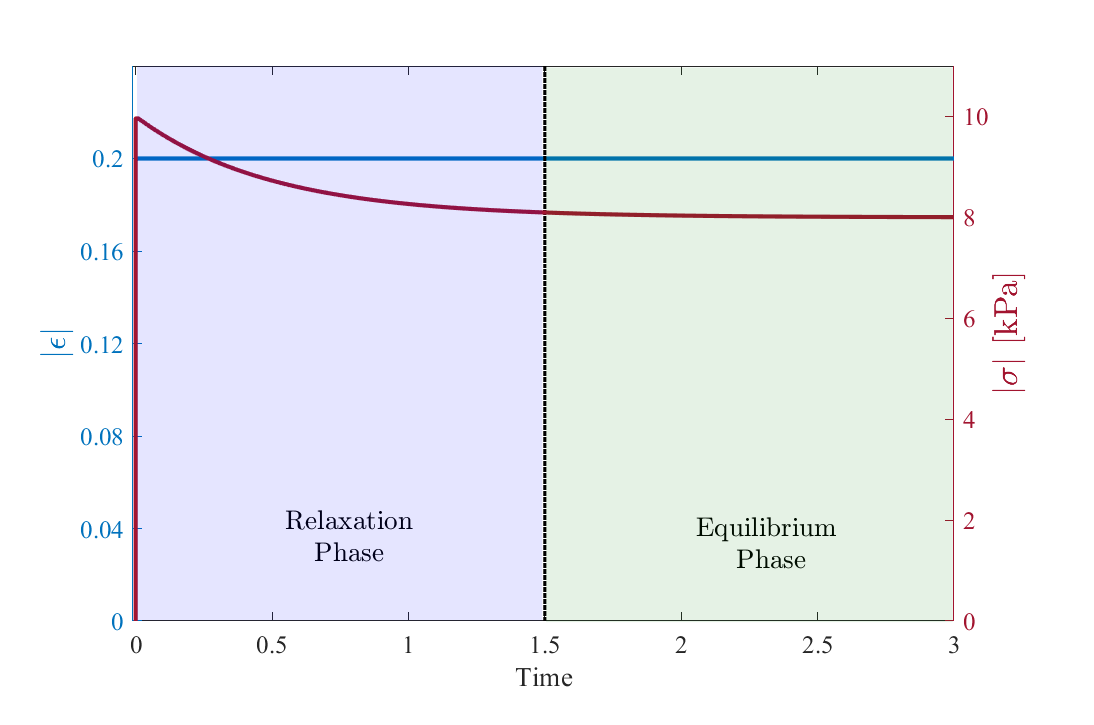
\includegraphics[scale=0.28]{images/SLS}\qquad 
	\caption{}
	\end{subfigure}

\vspace{5mm}
\begin{equation}
\begin{cases}
\sigma = E_1\epsilon+E_2\epsilon_d\\
\dot{\epsilon}_e = \dot{\epsilon} -\frac{E_2}{\eta} \epsilon_e = \dot{\epsilon} - \frac{\epsilon_e}{\tau_R}
\end{cases}
\tag{SLS}
\end{equation}
\vspace{3mm}
\caption{1D Standard Linear Solid. (a) Rheological Model; (b) Standard Response to a compression test. (1) Differential Equation for the Standard Linear Solid model in the 1D case.}
\label{SLS}
\end{figure}

In the framework of large deformation, a standard approach to the study of couple phenomena is the use of a multiplicative decomposition of the deformation gradient. We will be rely on the same idea to build our poro-visco-elatic model. In the literature of soft matter, two possible decomposition have been proposed, based on arbitrary choice, but never systematically compared. As our analysis shows, multiplicative decomposition should be treated as constitutive laws of the material and thus validated  and compared. Instead of arbitrarily choosing one of the two, we here develop both approaches, with the aim of identifying their differences and investigating experimental result which would allow us to experimentally test which one best describes the behaviour of soft tissues. 

Our work is organized as follows: in Section \ref{ECMcomp}, we discuss more in details the composition of the ECM. We then present a brief overview of Classical Irreversible Thermodynamics, which focuses on the principles later used in the derivation of our model in Section \ref{modeldev}. Common  [... FOLLOWING SECTIONS TO UPDATE AS I WRITE.]

\section{Composition of Extracellular Matrix.}
\label{ECMcomp}
Despite the tissue-specific nature of Extracellular Matrix (ECM), this is usually composed of a network of collagen fibrils entangled with proteoglycans (PGAs) which are covalently bonded to charged chains of glycosaminoglycans (GAGs), see Figure \ref{ECMfig_a}.  While collagen is mainly responsible for the mechanical behaviour of the tissue, GAGs can imbibe water, giving the extracellular matrix the ability to swell while maintaining its structural integrity. As mentioned in the introduction, from this point of view, the ECM is a polyelectrolyte gel. As schematically illustrated in Figure \ref{ECMfig}(b), polyelectrolyte gels are 3D networks of cross-linked polymer chains that contain ionizable functional groups. When in solution the gel swells, while the functional groups dissociate into fixed charges and mobile ions in the solution.  In particular, research has been focusing on the phenomena of swelling, i.e. large deformation due to absorption of water, and the diffusion transport and release of solution  \cite{DROZDOV+,DROZDOVph,Reviewpolyel,swell2}. However, only a small fraction of the study published accounts for the visco-elastic properties of the polymer network.

\begin{figure}[h]
	\begin{subfigure}{0.49\textwidth}
		\centering
		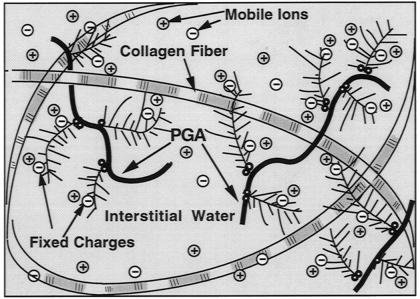
\includegraphics[scale=0.38]{images/ECM}
		\caption{}
		\label{ECMfig_a}
	\end{subfigure}
	\begin{subfigure}{0.49\textwidth}
		\centering
		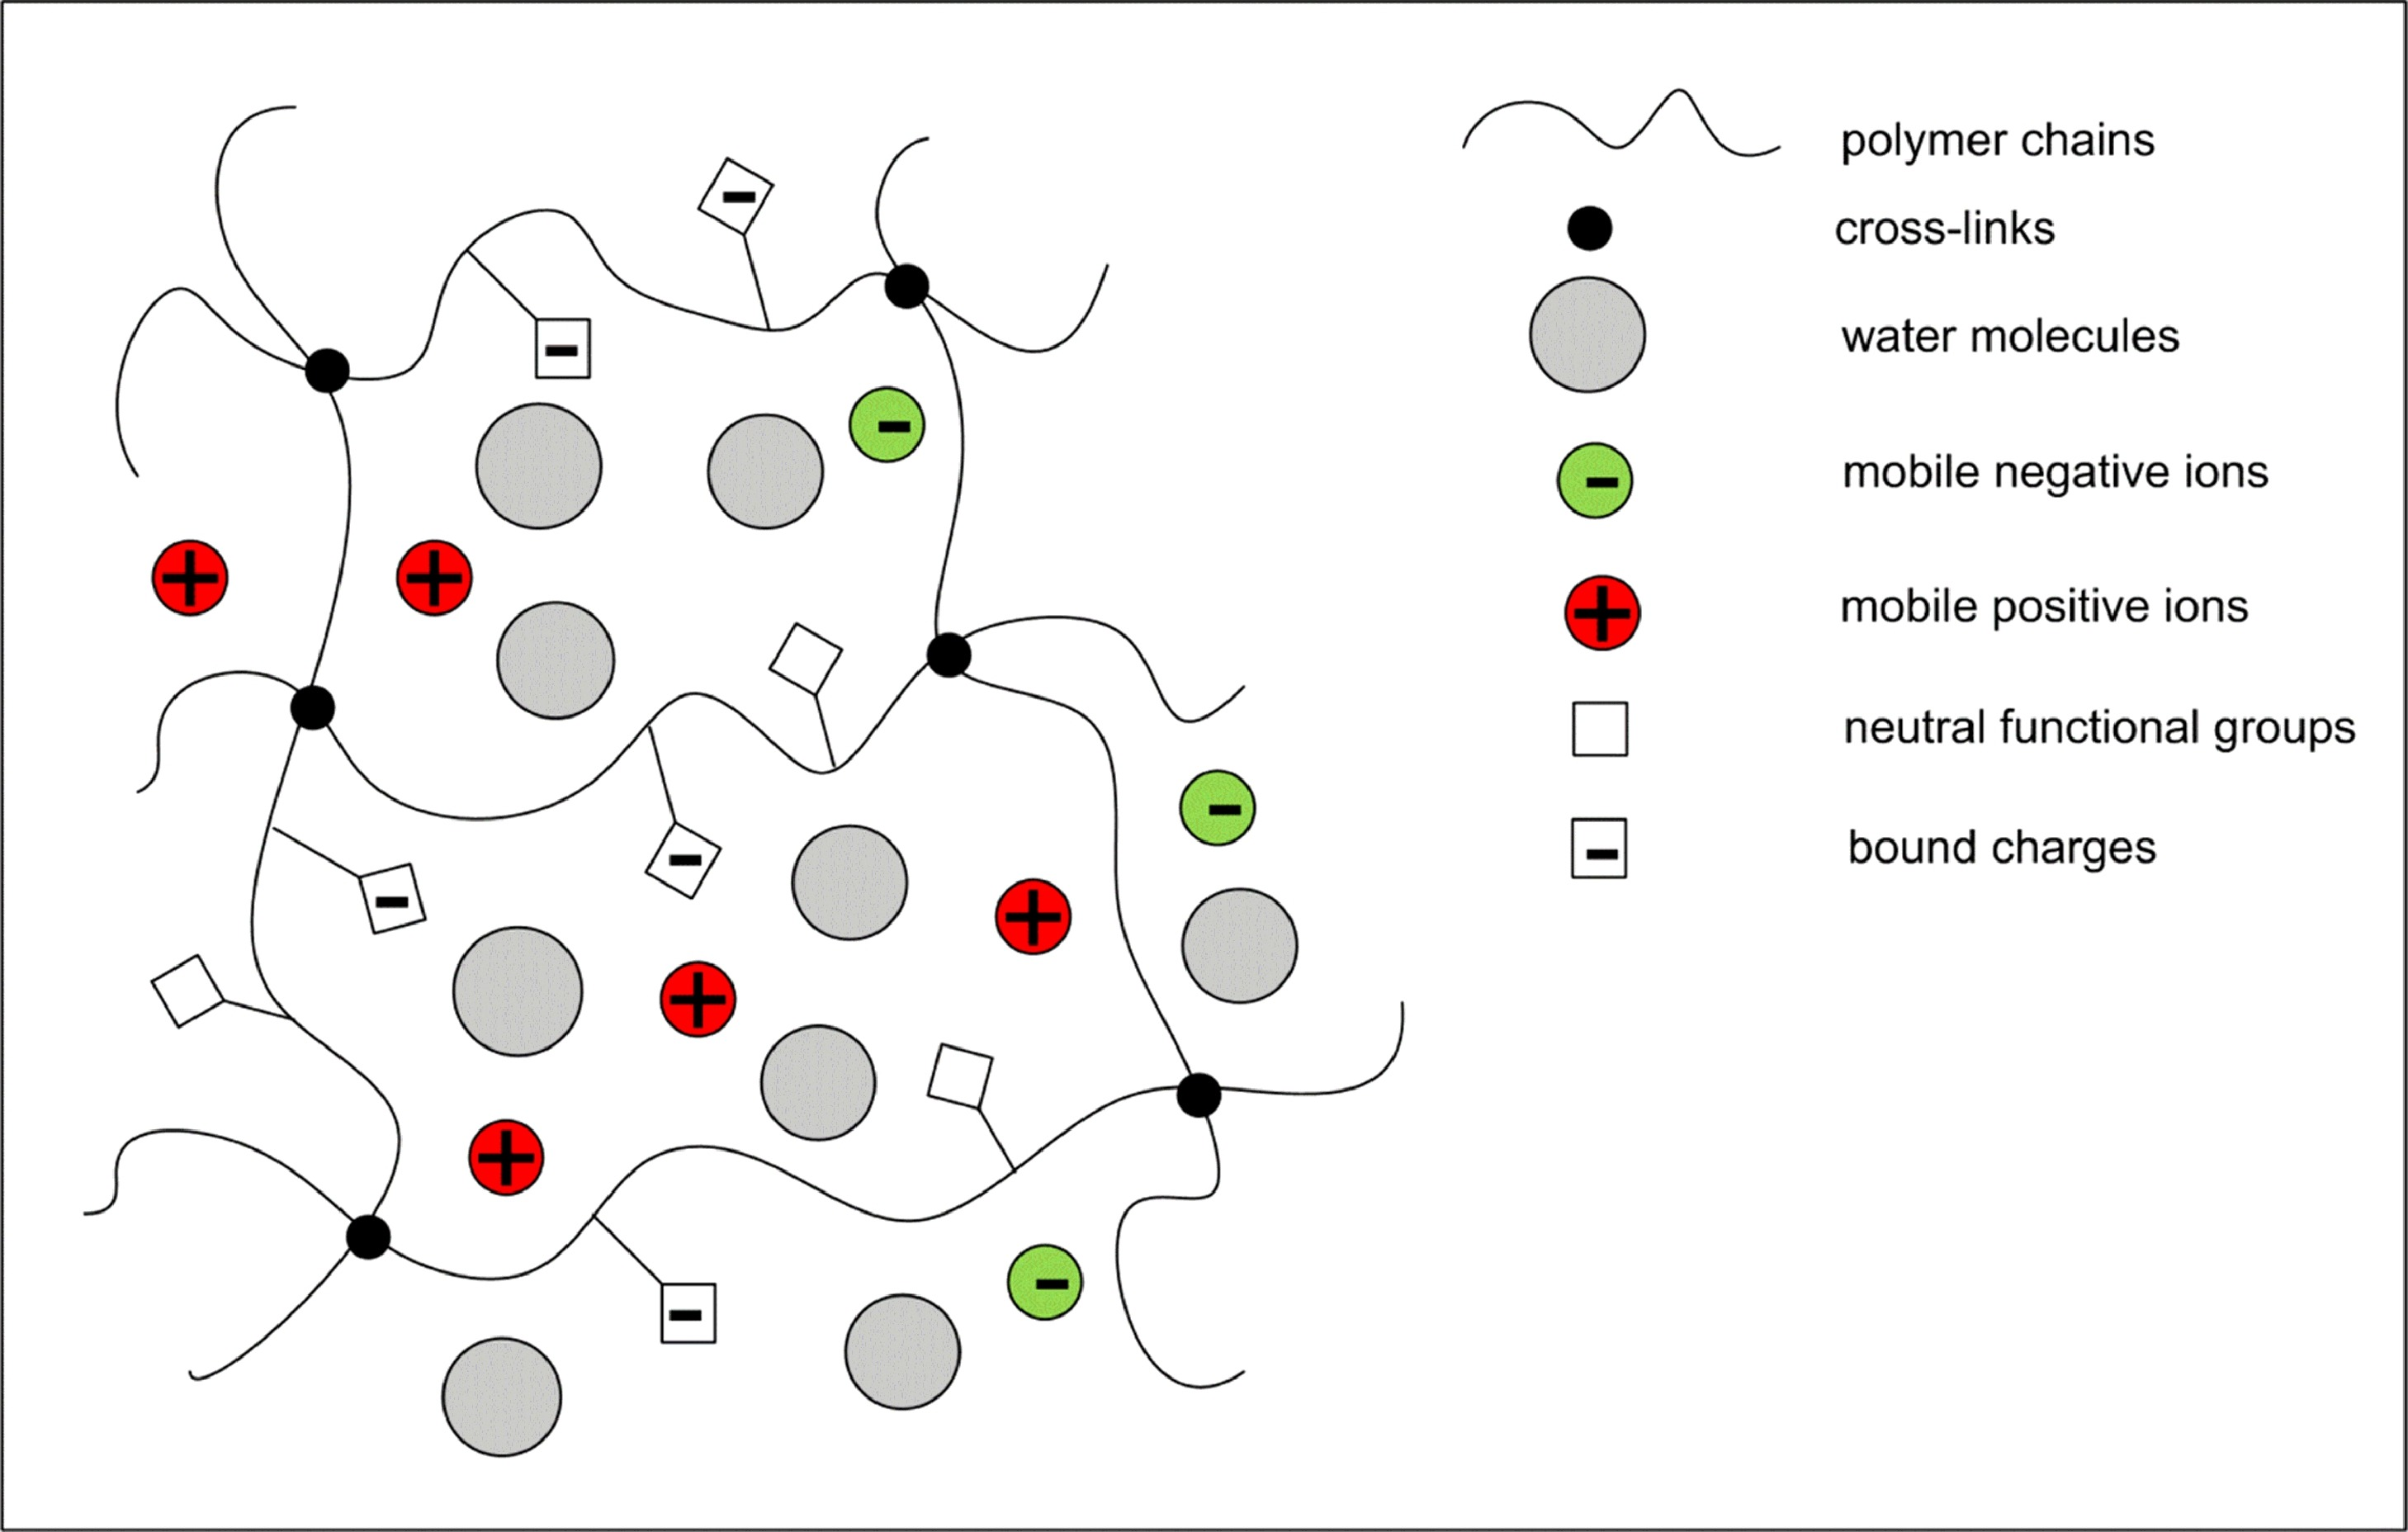
\includegraphics[scale=0.42]{images/ecmscheme.jpg}
		\caption{}
	\end{subfigure}
	\caption{Analogy between ECM in soft tissue and polyelectrolytes hydrogels: (a) schematic diagram of the structure of the charged hydrated articular cartilage, reproduced from \cite{pictureECM}; (b) an anionic polyelectrolyte gel modelled as a three-phase continuum, reproduced from \cite{DROZDOVph}.}
	\label{ECMfig}
\end{figure}

As shown in Figure \ref{ECMfig}, the extracellular matrix falls into the definition of polyelectrolytes so that the knowledge acquired in the study of these materials can be transferred to soft tissues. For the purpose of this study, we will not explicitly distinguish between collagen, PGAs and GAGs. At the tissue level, this can be grouped into a single solid phase (the polymer network), whose mechanical properties are treated as the average over the different components contribution. As is common in multiphase models of tissue, we will assume that the matrix is isotropic and GAGs are evenly distributed on the network. While this is not a good approximation for tissue like cartilage, which are highly anisotropic, it does apply to the extracellular matrix found in soft tissue such as liver, brain and tumours. It is also important to point out that ECM has additional properties such as thermo-sensitivity and pH-sensitivity. However, both in living organisms and in experimental set-up temperature and pH are maintained fairly constant.

\section{Non Equilibrium Thermodynamics.}
\label{secNET}
While equilibrium thermodynamics can describe ideal, i.e. reversible, processes, it does not apply to real processes which are irreversible. In this cases, the change in the entropy of a system $\d S$ results from both the reversible exchange of energy and matter with the external environment $\d_eS$ and the internal dissipation of energy during the process $\d_iS$ \cite{NET}:
\begin{equation}
\d S = \d_eS + \d_iS, 
\end{equation}
According to the second law of thermodynamics, which applies universally to any system or any of its sub-part $\d_i S\ge 0$. It is important to notice that the second law allows transformations in which total change in entropy $d S$ of the system is negative. This occurs whenever $-\d_e S>\d_i S$ and it can lead to the spontaneous formation of complex and ordered structures such as living organisms. From this point of view, life has emerged as an efficient mechanism able to increase sufficiently the entropy of its environment \cite{JeremyEngland}.  

In this study, we will focus on isothermal processes, i.e. $T=const$. Under this assumption, as derived by Gurtin in \cite{GURTIN}, the second law of thermodynamics is equivalent to the following \textit{energy imbalance inequality}:
\begin{equation}
\frac{\d}{\d t} \left\{\int_R \psi \right\}\leq W(R) + M(R) \label{energyin}
\end{equation}
where $R$ is a arbitrary control volume of the system, $\psi$ is the Helmholtz free energy, $W(R)$ is the rate at which the environment does work on $R$ and $M(R)$ is the inflow of mass due to transport. It is important to note that, as long as the quantities involved are well defined, the energy inequality~(\ref{energyin}) holds for any isothermal process independently of the specific physical system considered. This imposes a constraint on the form of the function $\psi$ and its dependence on the other thermodynamic variables, such as temperature or pressure, which are used to describe the system. 

Non-equilibrium thermodynamics mainly focuses on defining the form of $\d_i S$, which, unlike the reversible entropy production $\d_e S$, is not a state variable but depends on the specific transformation applied to the system. 
Different theories have been proposed, \cite{NET}, each with its assumptions and specific domain of applicability. In our study we will focus on \textquotedblleft Classical Irreversible Thermodynamics'' (CIT) which was pioneered by Onsager \cite{onsager} and Prigogine \cite{prigogine} in the first half of the 20th century. One the most important assumptions of this theory is the \textit{Local Equilibrium Hypothesis}, which guarantees thermodynamic variables, including entropy, are locally well-defined, \cite{NET}. 
Consequently, we can introduce the entropy density $s=s(\mathbf{x},t)$ such that:
\begin{equation}
S = \int_{R} s \,\d V, \qquad \d s = \d_e s + \d_is, \qquad \d_is > 0, 
\end{equation}
and the local entropy production:
\begin{equation}
\sigma \equiv \frac{\d_i s}{\d t} \geq 0.
\end{equation}

Another central aspect of the theory is the introduction of \textit{thermodynamic forces} \footnote{Not to be intended in the mechanical sense} $F_m$ (causes) and \textit{thermodynamic fluxes} $J_m$ (effects) to describe the time evolution of the system during an irreversible transformation. These are related to $\sigma$ as follows:
\begin{equation}
\sigma = \sum_m F_m J_m\geq 0.
\label{2law}
\end{equation}

While the local equilibrium hypothesis is at the basis of most theories of non-equilibrium thermodynamics, the following two hypotheses uniquely identify CIT:
\begin{itemize}
	\item[1.] \textit{Linear Relation between forces $F$ and fluxes $J$}:
	\begin{equation}
	J_m = \sum_k L_{mk} F_k,\label{lin}
	\end{equation}
	where the constant $L_{mk}$ are referred to as \textbf{phenomenological coefficients};
	\item[2.] \textit{Microscopic Reversibility}: time reversibility of processes at the micro-scale. 
\end{itemize}

Starting from these two principles, in his seminal paper \cite{onsager} Onsager derives the well-known \textit{Onsager Reciprocal Relation}:
\begin{equation}
L_{mk}=L_{km}.
\end{equation}

If we now consider an isothermal transformation in the framework of CIT, alongside with the energy imbalance inequality, we have that the following must hold:

\begin{equation}
W(R)+M(R)-\frac{\d}{\d t} \left\{\int_R \psi \right\} = T \int_R \sigma \,\d V\, ,
\label{eqCIT}
\end{equation}

In the past few decades, CIT has been applied successfully to the modelling of several physical phenomena of interest for engineers, physicists and applied mathematicians. However, its validity is limited to phenomena near-equilibrium, for which a linear approximation of the flux-force relation holds. The growing interest in more complex far-from-equilibrium phenomena has pushed toward the development of a more general framework for the study of a non-equilibrium phenomena. Since this goes beyond the purpose of our study, we will not discuss it further. We do, however, highlight the law of steepest entropy ascent, which, according to Beretta \cite{SEA2}, seems to emerge as the fourth fundamental law of nature. In the linear regime, this principle can be used to prove Onsager's reciprocal relation \cite{SEA1}, with no reference to the microscopic reversibility hypothesis, whose validity remains instead controversial \cite{CIT}.

\section{Model Development}
\label{modeldev}
\subsection{Conservation Law.}
\label{conslaw}
As mentioned in the previous section, we here consider the ECM as a three-phase medium composed of a solid polymer network with fixed charges, a solvent (i.e. water molecules, interstitial fluid) and solutes (freely moving charges). 
\begin{figure}[h!]
	\centering
	\def\svgwidth{0.9\linewidth}
	\input{latex/images/deformation.pdf_tex}
	\caption{Sketch of the dry and current state of the ECM network.}
	\label{Above}
\end{figure}

As the tissue deforms, the material element originally located at $\mathbf{X}$ in the initial configuration $\mathcal{B}_0$ is displaced to the point $\mathbf{x}$ in the current configuration $\mathcal{B}_t$, see Figure \ref{Above}. Such transformation is described by the deformation gradient tensor $\F= \partial \mathbf{x}/\partial \mathbf{X}$; the information about the change in ECM volume is encoded in $J= \det \F$. As in \cite{sarah}, we consider the reference, or initial, state $\mathcal{B}_0$, which is stress free, to be equivalent to the dry stage of the ECM, i.e. only solid phase present. Since we assume the solid phase to be incompressible, any change in the volume can only be related to the migration of solvent and solutes molecules, whose nominal concentrations will be denoted by $C_s$ and $C_i$ respectively, $i=1,\ldots,N$ with $N$ being the number of free ion species. This lead to the molecular incompressibility condition:

\begin{equation}
 J= 1 + v_s C_s +\sum\limits_{i=1}^{N} v_i C_i
 \label{comp}
\end{equation}
where $v_m$ are the characteristic molecular volume of each species in the solution. When considering the interstitial fluid, the contribution of ions to the volume can be neglected \cite{ecm1,ecm2} so that Equation~(\ref{comp}) reduces to:

\begin{equation}
J=1+v_s C_s.
\label{inc}
\end{equation} 

Consequently, the volume fractions of fluid $\phi_f$ and solid $\phi_n$ phases in the gel are defined as:
\begin{equation}
\phi_f = \frac{v_sC_s}{1+v_sC_s}, \qquad \phi_n = \frac{1}{1+v_sC_s}.
\end{equation}
where again we are neglecting the contribution of ions to the total volume.
While $C_m$ denote the number of each molecule per unit volume in the initial configuration for the $m$-th species in the solution, the actual concentration in the current state is denoted by $c_m=C_m/J$. Throughout the derivation of the model, we will be using the index $i=1,\ldots,N$ to denote the ionic species only, while $m\in\left\{s,1,\ldots,N\right\}$ refers to all mobile species, i.e. both the solvent and solutes.

Mass conservation must apply to all mobile species and in the initial configuration this reads:
\begin{equation}
\dot{C}_m + \nabla_0 \cdot \mathbf{J}_m = 0, \label{consmass}
\end{equation}
where $\mathbf{J}_m$ is the nominal flux per unit area in the dry state, $\dot{C}_m$ is the derivative of $C_m$ with respect to time, i.e.  $\dot{C}_m\equiv\partial_t C_m$ and $\nabla_0$ denote the gradient in the Lagrangian coordinates $\mathbf{X}$. Their counterparts in the actual configuration are denoted by $\mathbf{j}_m$ and $\nabla$ and are defined according to the following rules:
\begin{equation}
\mathbf{J}_m = J \F^{-1} \mathbf{j}_m, \qquad \nabla_0 (\cdot) = \F^{T} \nabla(\cdot).
\end{equation}

When considering tissues or hydrogels, inertial and gravitational effect are commonly neglected, so that the conservation of momentum for the ECM reads:

\begin{gather}
\nabla_0 \cdot \mathbb{S}=0\label{consmom},
\end{gather}

where $\mathbb{S}$ is the first Piola-Kirchoff tensor, which represents the stress state of the ECM in the initial configuration. The counterpart in the current configuration is the Cauchy stress tensor $\mathbb{T}$, which is related to $\mathbb{S}$ as follows:

\begin{equation}
\mathbb{T} = J^{-1}\mathbb{S}\F^T.
\end{equation}

The presence of free moving ions generates an electric field which is denoted by $\mathbf{E}$ and $\mathbf{e}$ in the initial and current configuration respectively. Introducing the electrostatic potential $\Phi$, we have that:
\begin{equation}
\mathbf{E}= -\nabla_0 \, \Phi, \hspace{8mm} \mathbf{e}= - \nabla \, \Phi.
\end{equation}

As in \cite{Reviewpolyel}, we consider the matrix to be a dielectric material\footnote{an electrical insulator, which can be polarized in the presence of an electric field.}. Consequently, the presence of the electric field generates an electric displacement $\mathbf{H}$\footnote{the vector field that accounts for both the electric field and the polarization of the dielectric material.}, which must obey Gauss law of electrostatics:
\begin{equation}
\nabla_0 \cdot \mathbf{H}= Q,
\label{gauss}
\end{equation}
where $Q$ is the local total charge, which accounts for both fixed and moving charges:
\begin{equation}
Q = e\left(\sum\limits_{i} z_i C_i+z_f C_{f}\right)\, , 
\end{equation}
where $e$ is the elementary charge, $C_f$ is the concentration of fix charges and $z_m$ is the valence of the corresponding charged species. Note that $C_f$ here corresponds to the concentration of GAGs, which is assumed to be a constant a fraction of $C_s$. As for above, we can move from nominal quantities to the corresponding value in the current configuration by applying the following rules:

\begin{eqnarray}
\mathbf{H} = J \mathbf{h}\F^{-T},\\
\mathbf{E} = \F^T \mathbf{e},
\end{eqnarray}
where $\mathbf{h}$ is the electric displacement in the current configuration.

\subsection{Kinematics.}
\label{kin}

As mentioned in the introduction, we model the ECM as a poro-visco-elastic material, with particular interest in the viscous aspect of the material. As shown in Figure \ref{deformation}, there are two molecular processes that give rise to the macroscopic time-dependent response of the system: 
\begin{itemize}
	\item [1.] the rearrangements of molecules at the micro-scale,  which has entropic origin and result in a volume-preserving viscous deformation;
	\item[2.] the long range transport of fluid that leads to swelling, i.e. changes in the ECM's size. 
\end{itemize}

\begin{figure}[h!]
	\hspace{-10mm}
	\def\svgwidth{1.2\linewidth}
	\input{latex/images/visco_poro.pdf_tex}
	\caption{Illustration of the molecular processes which account for the macroscopic deformation of ECM: viscosity is related to change in the conformation of the network which preserve the volume of the network.}
	\label{deformation}
\end{figure}
As illustrated in Figure \ref{deformation}, at the microscopic level this results in a visco-elastic and poro-elastic behaviour respectively.

In order to capture both phenomena, as common in the large-deformation theory \cite{Article1,CACCAVO2,Plasto,magneto,NGUYEN,growthtum} and first proposed by Kr\"{o}ner in 1960 \cite{kro}, we consider a multiplicative decomposition of the deformation tensor $\F$. As this can be choose arbitrary, different decomposition have been proposed in the literature. We will here consider the two most commonly used, which will be here denoting by model A \cite{Article1,CACCAVO2,Plasto} and model B \cite{magneto,NGUYEN,Jeru}:

\begin{gather}
\text{MODEL A} \Rightarrow\begin{cases}
\F=\F_e\F_v,\\
\det\F_v=1, \quad \det\F_e=\det\F
\end{cases} \label{dec1}\tag{A}\\[4pt]
\text{MODEL B} \Rightarrow\begin{cases}
\F= \F_{vol}\bar{\F}=\F_{vol}\bar{\F}_e\bar{\F}_v\\
\det\F=\det\F_{vol},\quad \det\bar{\F}=\det\bar{\F}_e=\det\bar{\F}_v=1.\label{dec2}
\end{cases}\tag{B}
\end{gather}

Comparing the two, we note that the only difference is that in model B the volumetric deformation, $\F_{vol}$, is decoupled from the deviatoric one, $\bar{\F}$.
To the best of our knowledge, there is no previous systematic study in the literature that compares these two approaches. While the two model are identical in the case of iso-volumetric deformation, i.e. $\det \F=J=1$, this is not always the case when a tissue swells. As it will be clear in Section \ref{excomp}, the choice of how to decompose the vector $\F$ is not only a mathematical argument but also affect the constitutive assumption on the material properties. This highlights the need of experimental testing to validate which model better describe the material studied.

As an explanatory example of the derivation of a model in the non-equilibrium thermodynamics framework, we will fully derive in the main text only the governing equation for model A. The interested reader can find the details of the derivation for model B in Appendix \ref{modelB}. 


%	\centering
%	\begin{subfigure}{0.32\textwidth}
%		\centering
%		\Large
%	\def\svgwidth{0.95\linewidth}
%	\input{latex/images/modelA1.pdf_tex}
%	\caption{Rheological Model A}
%	\label{fig1A}
%	\end{subfigure}
%\hspace{10mm}
%	\begin{subfigure}{0.32\textwidth}
%	\Large
%	\def\svgwidth{0.95\linewidth}
%	\input{latex/images/modelB1.pdf_tex}
%	\caption{Rheological Model B}
%	\label{fig1B}
%\end{subfigure}

\begin{figure}[h!]
	\centering
	\hspace{20mm}
	\Large
	\def\svgwidth{0.6\linewidth}
	\input{latex/images/modelA2.pdf_tex}\caption{multiplicative decomposition corresponding to model A, Equation~(\ref{dec1}).}
\label{Model2}
\end{figure}

Looking back at Equation~(\ref{dec1}), $\F_e$ is the elastic contribution to the deformation while, the term $\F_v$ accounts for the viscous flow. As illustrate in Figure \ref{Model2}, the multiplicative decomposition is equivalent to introducing an intermediate configuration $\mathcal{B}_v$, called the natural or virtual configuration. The evolution of the natural configuration can be interpreted as an entropy producing, i.e. dissipative, process. On the other hand, in the elastic deformation from the natural to the current configuration energy is only stored in the system. 

Using Equation~(\ref{dec1}), we can compute the velocity gradient tensor $\LL$:
\begin{equation}
\LL = \dot{\F}\F^{-1} = \LL_e + \F_e \LL_v \F_e^{-1},
\end{equation}
where $\LL_e=\dot{\F}_e\F_e^{-1}$ and $\dot{\F}_v\F_v^{-1}$ are respectively the elastic and viscous velocity gradient tensor. These can be decomposed in their symmetric $\mathbb{D}$ and skewed $\mathbb{W}$ part:

\begin{equation}
\begin{aligned}
\LL_e = \mathbb{D}_e + \mathbb{W}_e, \ \ \mathbb{D}_e = \frac{\LL_e+\LL^T_e}{2}, \ \ \mathbb{W}_e = \frac{\LL_e-\LL^T_e}{2};\\
\LL_v = \mathbb{D}_v + \mathbb{W}_v,  \ \ \mathbb{D}_v = \frac{\LL_v+\LL^T_v}{2}, \ \ \mathbb{W}_v = \frac{\LL_v-\LL^T_v}{2}.
\end{aligned}
\end{equation}

The decomposition~(\ref{dec1}) is not unique, as stress state in $\mathcal{B}_v$ would not change under any arbitrary rigid-body rotation \cite{multdec}. As suggested by \cite{Plasto}, in the case of isotropic material, it is reasonable to assume the viscous flow to be irrotational, i.e. $\mathbb{W}_v=\mathbb{O}$, so that $\LL_v \equiv \mathbb{D}_v$.
As mentioned before, the physical nature of the viscous deformation is molecular rearrangement so that volume is preserved. This requires to introduce the additional constraint:
\begin{equation}
J_v=\det \F_v= 1.\label{Jv}
\end{equation}

\subsection{Energy Balance Inequality.}
\label{sec_ine}

As mentioned in Section \ref{secNET}, according to how the system exchanges energy and mass with the environment, the energy imbalance imposes restrictions on the free energy $\psi$. Considering a control volume $R$ in the reference configuration $\mathcal{B}_0$, the system exchanges mass due to the diffusion of each mobile species, so that $M(R)$ is given by:
\begin{equation}
M(R)= \sum\limits_{m=s,1,\ldots,N} - \int_{\partial R} \mu_m \,\mathbf{J}_m \cdot \mathbf{n} 
\end{equation}
where $\mathbf{n}$ is the unit normal vector to the surface $\partial R$ and $\mu_m$ is the chemical potential associated with each species. Widely used in the thermodynamics of mixture, the chemical potential is a measure of the rate of change in free energy associated with adding one more molecule to a unit volume.

The term $W(R)$, i.e. the rate of work done on the system, is instead decomposed in two contributions, the rate of electrical $W_{el}(R)$ and mechanical work $W_{mec}(R)$. Following \cite{DROZDOVph}, $W_{el}(R)$ is defined as:
\begin{equation}
W_{el}(R) = -\int_{\partial R} \Phi\, \dot{\mathbf{H}}\cdot \mathbf{n}
\end{equation}

Following the work of Gurtin \cite{GURTIN}, we account both for the presence of macro-stresses $\mathbb{S}$ and micro-stresses $\boldsymbol{\xi}$, which arise due to the system heterogeneity \cite{microstress}. As before we only consider the dominant contribution of the solvent while neglecting the solute, so that $W_{mec}(R)$ reads:
\begin{equation}	\centering
%	\begin{subfigure}{0.32\textwidth}
%		\centering
%		\Large
%	\def\svgwidth{0.95\linewidth}
%	\input{latex/images/modelA1.pdf_tex}
%	\caption{Rheological Model A}
%	\label{fig1A}
%	\end{subfigure}
W_{mec}(R) = \int_{\partial R} \left(\boldsymbol{\xi}\cdot \mathbf{n}\right)\dot{C}_s + \int_{\partial R} \mathbb{S}\mathbf{n} \cdot \dot{\mathbf{u}}
\end{equation}
where $\mathbf{u}= \mathbf{x}-\mathbf{X}$ is the displacement vector, which is related to the deformation tensor by $\F=\mathbb{I}-\nabla_0 \mathbf{u}$. Substituting this result back into the formula~(\ref{energyin}) and applying the divergence theorem we obtain the following inequality:
\begin{equation}
\int_R \dot{\psi} - \mathbf{E}\cdot \dot{\mathbf{H}} \, + \, \sum\limits_{i=1}^{N} \left[e \Phi  z_i \dot{C}_i+ \nabla_0 \left(\mu_i \mathbf{J}_i \right)\right] + \nabla_0 (\mu_s \mathbf{J}_s- \boldsymbol{\xi}\dot{C}_s -\mathbb{S}^T\mathbf{\dot{u}}) \leq 0 
\end{equation}

Since this must hold for any choice of the volume $R$, the inequality must hold also locally:
\begin{equation}
\dot{\psi} - \mathbf{E}\cdot \dot{\mathbf{H}} \, + \, \sum\limits_{i=1}^{N} \left[e \Phi  z_i \dot{C}_i+ \nabla_0 \left(\mu_i \mathbf{J}_i \right)\right] + \nabla_0 (\mu_s \mathbf{J}_s- \boldsymbol{\xi}\dot{C}_s -\mathbb{S}^T\mathbf{\dot{u}}) \leq 0. 
\end{equation}
Further accounting for Equations~(\ref{consmass})-(\ref{consmom}), we obtain that:
\begin{equation}
\begin{aligned}
\dot{\psi} - \mathbf{E}\cdot \dot{\mathbf{H}} \, + \, \sum\limits_{i=1}^{N} \left[e \Phi  z_i - \mu_i\right] \dot{C}_i - (\mu_s + \nabla_0 \cdot \boldsymbol{\xi})\,\dot{C}_s -\mathbb{S}:\dot{\F}\\
-\boldsymbol{\xi} \cdot \nabla_0 \, \dot{C}_s + \sum\limits_{m} \nabla_0 \, \mu_m \cdot \mathbf{J}_m \leq 0.
\label{temp2}
\end{aligned} 
\end{equation}

As exhaustively discussed in previous studies \cite{Plasto,GURTIN}, the energy inequality imposes restrictions on the constitutive equation of the free energy $\psi$. Adapting their results to our specific problem, we have that:
\begin{equation}
\psi = \psi (\F,\F_e, C_s, C_i, \nabla_0 \,C_s,\mathbf{H}), \label{temp1}
\end{equation}
which precludes any explicit dependency of $\psi$ on the chemical potential or the viscous deformation gradient $\F_v$. By differentiating the incompressibility condition~(\ref{inc}) and~(\ref{Jv}), we obtain:

\begin{gather}
v_s\dot{C_s} - J \F^{-T}:\dot{\F} =0, \label{temp3}\\
\mathbb{I}:\LL_v=0. \label{temp4}
\end{gather}

If we now substitute~(\ref{temp1}) into~(\ref{temp2}), and include the constraint~(\ref{temp3})-(\ref{temp4}) using as Lagrange multipliers $p$ and $p_v$ respectively, we are left with the augmented form of the energy imbalance inequality:
\begin{equation}
\begin{aligned}
\color{blue}{\left(\frac{\partial \psi}{\partial \nabla_0 C_s}-\boldsymbol{\xi}\right)} \color{black}\cdot \nabla_0 \dot{C}_s + \color{blue}{\left(\frac{\partial \psi}{\partial C_s}-\mu_s-\nabla_0 \cdot \boldsymbol{\xi}+p v\right)}\color{black}\dot{C}_s\\
+ \sum_i\color{blue}\left(\frac{\partial \psi}{\partial C_i} + e\Phi z_i-\mu_i\right) \color{black}\dot{C}_i +\color{blue}\left(\frac{\partial \psi}{\partial \mathbf{H}}-\mathbf{E}\right) \cdot \color{black}\dot{\mathbf{H}}\\
+ \color{blue} \left(\frac{\partial \psi}{\partial \F} + \frac{\partial \psi}{\partial\F_e}\F_v^{-1}- \mathbb{S} - p J \F^{-T}\right): \color{black}\dot{\F}+ \sum_m \nabla_0 \,\mu_m \cdot \mathbf{J}_m \\
- \left(\F_e^T\frac{\partial \psi}{\partial \F_e}-p_v\mathbb{I}\right):\mathbb{L}_v\leq 0 . \label{ineq}
\end{aligned}
\end{equation}

Note that in deriving~(\ref{ineq}), we have also made us of the following identity:
\begin{equation}
\dot{\F}=\dot{\F}_e\F_v+\F_e\dot{\F}_v \Longrightarrow \dot{\F}_e=\dot{\F}\F_v^{-1}-\F_e \LL_v.
\end{equation}

\subsection{Construction of the Free Energy.}

Having the general form of $\psi$, Equation~(\ref{temp1}), it remains to construct its precise form. Following a standard approach in $\psi$-depending modeling, we assume that the total free energy can be additively decomposed with each physical mechanisms contributing independently. We here consider six distinct contributions:

\begin{enumerate}
	{\indentitem\item[\textbullet] the energy of the electric field $\psi_1$;}
	{\indentitem \item[\textbullet] the energy of solvent and solutes' molecules not interacting with the solid phase $\psi_2$;}
	{\indentitem\item[\textbullet] the energy of mixing the solid phase with the solution, $\psi_3$;}
	{\indentitem\item[\textbullet] the energy of mixing the solvent with the solutes in solution, $\psi_4$;}
	{\indentitem\item[\textbullet] the interfacial energy between dissimilar phases, $\psi_5$;}
	{\indentitem\item[\textbullet] the energy of the solid phase not interacting with the solution, $\psi_6$.}
\end{enumerate}

Assuming the solid phase to be an ideal and linear dielectric material, with constant permittivity $\epsilon$,the free energy of polarization reads \cite{DROZDOV+,Reviewpolyel}:
\begin{gather}
\psi_1 = \frac{1}{2\epsilon J} \mathbf{H}\F^T \cdot \F \mathbf{H}.
\end{gather}

The specific energy density $\psi_2$ has the standard form:
\begin{equation}
\psi_1 = \sum\limits_{m} \mu^0_m C_m
\end{equation} 
where $\mu^0_m$ denotes the chemical potential of non interacting solvent and ions molecules. According to Flory-Huggins theory \cite{flory,hug} of mixtures, the mixing energy is given by:
\begin{equation}
\psi_3 = \frac{k_B T J}{v_s} \left(\phi_f \ln \phi_f + \chi \phi_f \phi_n\right),\label{mix}
\end{equation}
where $k_B$ is the Boltzmann's constant, $T$ is the temperature and $\chi$ is the Flory-Huggins parameter, which is a measure of the enthalpy of mixing. Different is the approach of Xue et al. in \cite{ecm1,ecm2}. In these studies, the authors assume only the mixing of GAGs with solvent, while neglecting the collagen. Since we are considering GAGs and the collagen network as as a unique solid phase and we could not find any evidence that collagen does not mix with water, we have chosen the more general form~(\ref{mix}).

As the interstitial fluid is well approximated by a dilute solution, the contribution $\psi_4$ reads \cite{Reviewpolyel,ecm1,ecm2}:

\begin{equation}
\psi_4 = k_B T \sum\limits_{i=1}^{N} C_i \left(\ln \frac{C_i}{ C_s}-1\right).
\end{equation}

As proposed by Hong et al. \cite{Interface}, we include in the energy the effect of interface tension. Despite having been neglected in many models for hydrogel swelling, this term plays a role in the transient poroelastic relaxation of the material, when boundaries between solvent-rich and solvent-poor regions can emerge \cite{sarah,Interface}. Again we assume that the contribution of mobile ions is negligible, so that only the solid-solvent interface contributes to the energy:
\begin{equation}
\psi_5 = \frac{\gamma}{2} J \left|\nabla C_s\right|^2,
\end{equation}
where the constant $\gamma$ plays a role analogous to a surface tension.

Finally, we need to specify the strain energy $\psi_6$ which depends on the particular constitutive model used to describe the material. As mentioned in the Introduction the Standard Linear Solid (SLS), see Figure \ref{SLS}, is commonly used to describe soft material in the regime of small deformation. However, when account for large deformation, as in the case of swelling, soft material present a non-linear behaviour. For this reason we consider the model in Figure \ref{fig1A}, which is a generalization of the 1D SLS to 3D problems with non-linear elastic response. 

\begin{figure}
		\begin{subfigure}{0.32\textwidth}
			\centering
			\large
		\def\svgwidth{0.9\linewidth}
		\input{latex/images/modelA1.pdf_tex}
		\caption{}
		\label{fig1A}
		\end{subfigure}
	\hspace{20mm}
			\begin{subtable}{0.375\textwidth}
				\hspace{-15mm}
			\begin{tabular}{|c | c | c|}	
				\hline
				\multirow{2}{*}{\textbf{ Element } }& \textbf{ Constitutive } & \multirow{2}{*}{\textbf{ Deformation }} \\
				& \textbf{Properties} &\\
				\hline	
				 \multirow{2}{*}{ spring 1 } & Isotropic  & volumetric\\
				 &Neo-Hookean spring& + deviatoric\\
			 	\hline
				\multirow{2}{*}{ spring 2 } & Isotropic  & volumetric\\
				&Neo-Hookean spring &+ deviatoric\\ 
				\hline
				\multirow{2}{*}{dashpot}  & Isotropic  & 	\multirow{2}{*}{deviatoric}\\
				& Linear dashpot & \\
				\hline
			\end{tabular}
			\caption{}
		\end{subtable}
	\caption{(a) Schematic representation of the non-linear rheological model for ECM; (b) Table summarizing the major properties of the model components.}
\end{figure}

The strain energy can thus be decomposed into the sum of the contributions from spring $1$ and spring $2$:

\begin{equation}
\psi_6 = \psi_1(\F) + \psi_2(\F_e).
\end{equation}

As in \cite{ecm2}, we consider the spring to be isotropic and hyper-elastic (Neo-Hookean) which are characterised by the following form of the free-energy:

\begin{eqnarray}
\psi_1(\F) = \frac{G^A_1}{2} \left(\F:\F - 3 -2 \ln J\right)\\
\psi_2(\F_e) = \frac{G^A_2}{2} \left(\F_e:\F_e - 3 -2 \ln J_{e}\right)\label{hyp}
\end{eqnarray}
where $G_\mathbf{\cdot}$ stands for the shear modulus associated with each spring, $J_e= \det \F_e$, while $J$ is as defined in the previous sections. As derived in \cite{floryprinciples}, the hyper-elastic model~(\ref{hyp}) can be correlated to the microscopic properties of a polymer network, under the assumption of Gaussian chains and affine deformation. Other thermodynamically consistent form of the stretching energy have been proposed in the literature \cite{BERGSTROM1998931,boyce2,doi}. These have been also derived by statistical arguments but starting from different network models.

\subsection{Entropy Production $\sigma$.}
\label{ent}

Having specified how the system interacts with its environment, we can now discuss how it dissipates energy. As mentioned in Section~(\ref{kin}), there are two contributions: transport (diffusion of solvent and solutes) and viscosity. The thermodynamic fluxes \footnote{See Section \ref{secNET}} associated with these two phenomena are $\mathbf{J}_m$, $m=s,1,\ldots,N$, and $\LL_v$. Consequently, using Equation~(\ref{2law}), we obtain:

\begin{equation}
\sigma = \sum_m \zeta_m \cdot \mathbf{J}_m + \zeta_v : \LL_v,
\label{dis}
\end{equation}
where $\zeta$s represent the thermodynamic forces associate with each flux. On the other hand, $\nabla_0 \dot{C}_s$, $\dot{C}_s$, $\dot{C}_i$, $\mathbf{\dot{H}}$ and $\dot{\F}$ describe the evolution of reversible process. This implies that their value can be controlled and arbitrarily chosen, by carefully tune the condition of an experiment, while the energy imbalance inequality~(\ref{ineq}) continue to hold. Given the constraint~(\ref{temp1}) on $\psi$, this can only happen if the terms highlighted in blue in Equation~(\ref{ineq}) are identically zero. As shown in the Appendix [TO DO], this leads to the following system of equations:
\begin{gather}
\boldsymbol{\xi} = \gamma J \,\mathbb{B}^{-1} \,\nabla_0 \,C_s,\label{sys1}\\[2mm]
\begin{aligned}
\mu_s = p v_s + \mu_s^0 - \gamma J \nabla^2 C_s + k_BT&\left[\ln \frac{C_s v_s}{1+C_s v_s} + \frac{1}{1+C_sv_s}\right.\\
&\left.\ \ \ \ \ \ +\frac{\chi}{(1+C_s v_s)^2}-\sum_i \frac{C_i}{C_s}\right], 
\end{aligned}\label{gov1}\\[2.5mm]
\mu_i = \mu^0_i + e\Phi z_i + kT \ln \frac{C_i}{C_s},\label{mu}\\
\mathbf{E} = \frac{1}{\epsilon J} \F^T \F\, \mathbf{H}\, , \qquad -\epsilon J \nabla^2 \Phi = Q\, ,\label{sys2}
\end{gather}
\begin{gather}
\begin{aligned}
\mathbb{T}= -p \mathbb{I} + \underbrace{\gamma \left[\frac{1}{2} |\nabla C_s|^2\mathbb{I} - \nabla C_s \otimes \nabla C_s\right]}_{\mathbb{T}^{kort}}+ \underbrace{\epsilon \left[\frac{1}{2} \,|\nabla \Phi|^2\mathbb{I} -\nabla \Phi \otimes \nabla \Phi\right]}_{\mathbb{T}^{Max}}\\
+ \frac{G^A_1}{1+C_sv_s}\left(\mathbb{B}-\mathbb{I}\right) + \frac{G^A_2}{1+C_sv_s}\left(\mathbb{B}_e-\mathbb{I}\right),
\end{aligned}
\label{sys3}
\end{gather}

As discussed in Section \ref{secNET}, in the framework of linear non-equilibrium thermodynamics, when considering isothermal transformation, the second law of thermodynamics can be rewrite as Equations~(\ref{eqCIT}). Using the same argument as in Section \ref{sec_ine} and Equation~(\ref{dis}), we can rewrite Equations~(\ref{eqCIT}) in differential form, and substituting Equations~(\ref{sys1})-(\ref{sys3}), we obtain:
\begin{equation}
\begin{aligned}
 \sigma = -  \sum_m \frac{1}{T}\nabla_0 \,\mu_m \cdot \mathbf{J}_m + \frac{1}{T}\left( \F_e^T\frac{\partial \psi}{\partial \F_e}-p_v\mathbb{I}\right):\mathbb{L}_v\label{EQen}
\end{aligned} 
\end{equation}

Equating Equation~(\ref{EQen}) and~(\ref{dis}), it is evident that the thermodynamics forces are:
\begin{gather}
\zeta_m = \frac{1}{T} \nabla_0 \,\mu_m, \label{vflow1}\\
\zeta_v = \frac{1}{T} \left( \F_e^T\frac{\partial \psi}{\partial \F_e}-p_v\mathbb{I}\right) = \frac{1}{T} \left[G^A_2(\mathbb{C}_e-\mathbb{I})-p_v\mathbb{I}\right].
\end{gather}
Assuming to be in regime of linear non-equilibrium thermodynamics, we can use the identity~(\ref{lin}) to couple fluxes and forces. However, considering the symmetry constraint from \textit{Curie's law}\footnote{Macroscopic causes can not have more element of symmetries than the effect they cause \cite{CIT}} , there can be no coupling between fluxes and forces of different tensorial nature. Consequently, we are left with the following force-flux relation:
\begin{gather}
\LL_v = L_{vv} \zeta_v,\label{vflow2}\\
\mathbf{J}_m = \sum_{k=s,1,\ldots,N} L_{mk} \zeta_k. \label{dif}
\end{gather}

%Combining Equation~(\ref{vflow1}) and (\ref{vflow2}), and imposing that condition~(\ref{Jv}) is satisfied, we can characterise the viscous flow by the following relation:
%\begin{equation}
%\LL_v = L_{vv}T^{-1}\text{DEV}\left[\F_e^T\frac{\partial \psi}{\partial \F_e}\right] = \eta^{-1}\text{DEV}\left[\F_e^T\frac{\partial \psi}{\partial \F_e}\right] ,
%\end{equation}
%where $\eta$ represent the viscosity of the material and $\text{DEV}\left[\cdot\right] = \cdot-1/3\, \text{tr}(\cdot)$ is the deviatoric component of the tensor in the brackets. 

%The dissipative contribution due to the relative movement of phases has been largely studied in the literature \cite{ecm1,ecm2}. Starting from Equation~(\ref{dif}) and standard arguments we can get to the following definition for the fluxes:
As described in Appendix \ref{apenergy}, starting from Equations~(\ref{vflow1})-(\ref{dif}) and with common consideration from the theory of mixture, we can derive the following system of time dependent equations:
\begin{eqnarray}
\partial_t C_s=\nabla_0 \cdot\left[K C_s \F^{-1}\left(c_s\nabla \mu_s +\sum_i \frac{D_i}{D^0_i} c_i \nabla \mu_i\right)\right],\label{gov2}\\
\partial_t C_i= \nabla_0\cdot\left[\frac{D_i}{k_B T}C_i\F^{-1}\nabla \mu_i -\frac{D_i}{D^0_i} \frac{C_i}{C_s} \mathbf{J}_s\right],\label{gov3} \\
\dot{\mathbb{B}}_e =\LL\mathbb{B}_e + \mathbb{B}_e \LL^T - \frac{1}{\tau_R} \,\mathbb{B}_e\text{DEV}[\mathbb{B}_e].\label{Be}
\end{eqnarray}
where the parameters are macroscopic phenomenological coefficients, that can either be estimated experimentally or derived from the nano/microscopic properties of the different phases \cite{ecm1,ecm2}. To sum up the governing equations for the Model A are Equations~(\ref{gov1})-(\ref{sys3}) together with the flow rules~(\ref{gov2})-(\ref{Be}). The analogous system of equation for model B can be found in Appendix \ref{modelB}. 

\subsection{Evolution Equation.}

In order to get a better physical insight into the behaviour, we first rewrite the solvent chemical potential as:
\begin{gather}
\mu_s = \mu^0_s + k_B T \left(\frac{p v_s}{k_BT} +\Pi_{osm}-\sum_i \frac{C_i}{C_s} -\frac{\gamma J}{k_B T}\Pi_{grad}\right)\label{mu2},\\
\Pi_{osm}=\ln \frac{C_s v_s}{1+C_s v_s} + \frac{1}{1+C_sv_s}+\frac{\chi}{(1+C_s v_s)^2},\\
\Pi_{grad} = \nabla^2 C_s,
\end{gather}
where $p$ represents the pore pressure, $\Pi_{osm}$ is the osmotic pressure of the solution and $\Pi_{grad}$ is the pressure due to interface energy. If we now substitute into Equations~(\ref{gov2}) the chemical potentials~(\ref{mu2})-(\ref{mu}), which yields to:
\begin{equation}
\begin{aligned}
\partial_t C_s=\nabla_0 \cdot\left\{K\F^{-1}\left[C_s v_s\nabla p - \color{red}\gamma C_s J\nabla \Pi_{grad}\color{black}+\sum_i \frac{D_i}{D^0_i} C_i e z_i \nabla \Phi\right.\right.\\
\left.\left.+ k_B T\color{teal} \left(C_s \nabla \Pi_{osm}+ \sum_i\left(1-\frac{D_iC_i}{D^0_iC_s}\right) \nabla C_s - \sum_i\left(1-\frac{D_i}{D^0_i}\right) \nabla C_i \right)\color{black}\right]\right\}.\label{long}
\end{aligned}
\end{equation}

The above equation shows that the solvent transport is driven by pressure gradient, osmotic pressure gradient (green term in Equation~(\ref{long})), electric potential gradient and the additional composition gradient (red term in Equation~(\ref{long})), which is here first introduced in the context of polyelectrolytes. In the absence of solutes ($C_i\equiv 0$), we recover the same model presented by Hennessy et. al~\cite{sarah}. If we further assume that $|\nabla \Pi_{grad}|<<1$ and take the limit $v_sC_S\rightarrow\infty$, Equations~(\ref{long}) reduces to Darcy's law for the flow in a porous media. The model for polyelectrolytes proposed by Hong \cite{Reviewpolyel} correspond instead to the limit $D^0_i\rightarrow\infty$, i.e. mobile species can move freely in pure solution, and  $|\nabla \Pi_{grad}|<<1$.

Similarly we can rewrite Equation~(\ref{gov3}) as:
\begin{equation}
\scriptsize
\partial_t C_i = \nabla_0 \left[D_i\F^{-1}\left(\underbrace{\nabla C_i}_{\text{diffusion}} +\underbrace{\frac{eC_iz_i}{k_B T} \nabla \Phi}_{\text{electric}}\right)-\underbrace{\frac{D_i C_i}{C_s}\F^{-1}\nabla C_s}_{\text{osmotic pressure}}-\underbrace{\frac{D_i C_i}{D^0_iC_s}\mathbf{J}_s}_{\text{advenction}}\right]\label{long2}
\end{equation}

In the case of ions, the driving forces of transport are the diffusion of ions, the electric field, the osmotic pressure due to the mixing with the solvent and the advection term (due to the relative movement of ions with respect to the solvent). In the limit $D^0_i\rightarrow0$, where the ions can freely move in the pure solution, we recover the formulation of Hong in \cite{Reviewpolyel}, which is commonly used in the description of polyelectrolytes. In the dilute limit, i.e. when the concentration of ions is much smaller than the solvent  concentration $C_i<<C_s$, we can drop both the osmotic and advection term so to recover the well-known Nernst-Planck equation \cite[see Equation (6.67)]{Reviewpolyel}.

As mentioned in the introduction, one the major aspect of interest is the visco-elastic contribution to the evolution of the system. Even though in the transport Equation~(\ref{long})-(\ref{long2}) there is no direct reference to it, the transport is indirectly coupled to the visco-relaxation through the pressure gradient. Taking the divergence of Equation~(\ref{sys3}) and using the conservation of momentum~(\ref{consmom}), we can identify components to the pressure gradient:

\begin{equation}
\nabla p= \nabla \cdot \mathbb{T}^{kort} + \nabla \cdot \mathbb{T}^{Max} + G_1^A\underbrace{ \nabla \cdot \left[\frac{\B-\mathbb{I}}{1+v_sC_s}\right]}_{\substack{\text{swelling}\\\text{+ deviatoric}\\\text{ deformation}}} + \,\color{red} G_2^A \underbrace{\nabla \cdot\left[\frac{\B_e-\mathbb{I}}{1+v_sC_s}\right]}_{\color{black}\substack{\text{swelling}\\\text{+ deviatoric}\\\text{deformation}\\\text{+ viscous relaxation}}}\color{black}
\end{equation}

Differently from the standard Neo-Hookean model for polyelectrolytes, we have an additional term highlighted in red, which accounts for the energy stored in the second spring of model A. Its time evolution, as determined by Equation~(\ref{Be}) is driven by the swelling and macroscopic deformation and a relaxation term which capture the viscous nature of the solid phase:
\begin{equation}
\dot{\mathbb{B}}_e=\underbrace{\LL\mathbb{B}_e + \mathbb{B}_e \LL^T}_{\substack{\text{swelling}\\\text{+ deviatoric}\\\text{deformation}}} - \underbrace{\frac{1}{\tau_R} \,\mathbb{B}_e\text{DEV}[\mathbb{B}_e]}_{\substack{\text{viscous}\\\text{relaxation}}}\label{Be2}
\end{equation}


Despite the introduction of the non-linear terms, there is an apparent analogy between the above Equation and the ODE describing the standard linear solid, see Equation~(SLS) in the Introduction. The term $\dot{\epsilon} \leftrightarrow \LL$ is related to the strain experienced by spring 1, while $\epsilon_e  \leftrightarrow \mathbb{B}_e$ is the variable describing the strain on the 2. In the limit $\tau_R\rightarrow \infty$, we have that $\mathbb{B}_e\equiv\mathbb{B}$. We thus recover the standard Neo-Hookean hyper-elastic model for hydrogels with shear modulus given by $G^A_1+G^A_2$. Similar result are obtained for model B. The governing equation of Model B is equivalent to~(\ref{Be2}), except for the fact that it is not influence by purely volumetric deformation:
\begin{equation}
\dot{\bar{\mathbb{B}}}_e=\underbrace{\bar{\LL}\bar{\mathbb{B}}_e + \bar{\mathbb{B}}_e \bar{\LL}^T}_{\substack{\text{deviatoric}\\\text{deformation}}} - \underbrace{\frac{1}{\tau_R} \,\bar{\mathbb{B}}_e\text{DEV}[\bar{\mathbb{B}}_e]}_{\substack{\text{viscous}\\\text{relaxation}}}
\end{equation}
while the pressure gradient is defined as:
\begin{equation}
\begin{aligned}
\nabla p= \nabla \cdot \mathbb{T}^{kort} + \nabla \cdot \mathbb{T}^{Max} + G_1^B\underbrace{ \nabla \cdot \left[\frac{\text{DEV}[\bar{\mathbb{B}}]}{1+v_sC_s}\right]}_{\substack{\text{+ deviatoric}\\\text{ deformation}}} \\
+ \,\color{red} G_2^B \underbrace{\nabla \cdot\left[\frac{\text{DEV}[\bar{\mathbb{B}}_e]}{1+v_sC_s}\right]}_{\color{black}\substack{\text{ deviatoric}\\\text{deformation}\\\text{+ viscous relaxation}}}\color{black}+ G_{vol}\underbrace{\nabla \left(\frac{J^{2/3}-1}{J}\right)}_{swelling}.
\end{aligned}
\end{equation}

As we will discuss in the next section, when considering instead a purely volumetric deformation, such as for free swelling, i.e. $\F=\F_{vol}=J^{1/3}\mathbb{I}$, we have that the two model are equivalent given that $G_{vol}\equiv G_A +G_B$. Before comparing the model in different experimental setting, we have briefly summarised in Table~(\ref{summary}) the variables and governing equation for both models. In order to have a close solution, the proper boundary and initial conditions needs also to be assigned depending on the specific problem considered.

\vspace{3mm}
\begin{table}
	\centering
	\begin{tabular}{c|c|c}
		\hline\addlinespace[2pt]
		Variable &  \hspace{1pt} Model A \hspace{1pt} & \hspace{1pt} Model B\hspace{1pt} \\
		\hline
		\hline\addlinespace[2.5pt]
		Solvent Concentration &  \multicolumn{2}{c}{$C_s$~(\ref{long})}\\[2.5pt]
		Chemical Potential of & \multicolumn{2}{c}{ $\mu_s$~(\ref{gov1})}\\
		the solvent &\multicolumn{2}{c}{}\\[2pt]
		Ionic Concentrations &\multicolumn{2}{c}{$C_i$~(\ref{long2})}\\[3pt]
		Chemical Potential of & \multicolumn{2}{c}{$\mu_i$~(\ref{mu}) }\\
		the ions &\multicolumn{2}{c}{ }\\[2pt]
		\hline\addlinespace[2pt]
		Local Volumetric Change & \multicolumn{2}{c}{$J$~(\ref{inc})}\\[2.5pt]
		Cauchy Stress Tensor & 	\multicolumn{2}{c}{$\mathbb{T}$~(\ref{consmom})}\\[2.5pt]
		Deformation Gradient & $\F$~(\ref{dec1})& $\F$~(\ref{dec2})\\[2.5pt]
	 	Pore Pressure & $p$~(\ref{sys3}) & $p$~\ref{sys2B})\\[2.5pt]
		Left-Cauchy Tensor& \multirow{2}{*}{$\mathbb{B}_e$~(\ref{Be})} & \multirow{2}{*}{$\mathbb{\bar{B}}_e$~(\ref{BeB})}\\
		for spring 2&&\\
		Viscous Velocity & \multirow{2}{*}{$\LL_v$~(\ref{Lv1})}&  \multirow{2}{*}{$\bar{\LL}_v$~(\ref{Lv2})}\\
		Gradient Tensor&&\\
		\hline\addlinespace[2pt]
		Electric Field & \multicolumn{2}{c}{$\Phi$~(\ref{sys2})}\\
		\hline 
		\hline
	\end{tabular}
\vspace{3mm}
\caption{List of Variables involved in the problem, with reference to the corresponding governing equations.}
\label{summary}
\end{table}

\section{Elasticity: Equilibrium Behaviour.}
In this section, we will be focusing on the equilibrium behaviour of the two model under free and compressed swelling. Given the large number of parameter in the models, such experiment allows to estimate a subset of them. While previous model proposed in the literature have been arbitrarily chosen how to decompose the deformation gradient $\F$, we here shows that such choice need to consider equal to a constitutive equation and thus tested experimentally. 

\subsection{Unconstrained Free Swelling.} 
\label{free}
\begin{figure}
	\centering
	\def\svgwidth{0.95\linewidth}
	\input{latex/images/freeswell.pdf_tex}
	\caption{Schematic representation of a free swelling. Since we are considering an isotropic mixture, the ECM maintains its shape while all dimension are stretched of the same amount $\lambda$. So that the relative volume change is $\delta V = \lambda^3-1$. }
\end{figure}

Having derived the set of equations for both model A and model B, we now want to compare how the two behave in different settings. We first look at unconstrained free swelling of a cuboid slice of ECM immersed in a bath of interstitial fluid. For simplicity we consider that contains only two species of free ions, which carry a positive $C_+$ and a negative $C_-$ charge respectively. We assume the bath to be well-mixed and stress-free with both pressure and electric potential identically zero. We denote by $2c_0$ the total concentration of free ions in the bath, so that $c_0$ is the concentration of each ionic species. As the system evolves, the ECM increases in size until it reaches a steady state which is characterised by the continuity of chemical potentials and stresses across the boundary:
\begin{equation}
\left[\mu_s\right]^+_-=\left[\mu_+\right]^+_-=\left[\mu_-\right]^+_-=0, \quad \left[\mathbf{n} \mathbb{T}\mathbf{n}\right]^+_-=0.
\end{equation}

As in \cite{DROZDOVph}, we consider that at equilibrium the following conditions also holds:
\begin{itemize}
	\item[1.] chemical potentials of solvent and solutes is homogeneous and equal in the bath and in the bath:
	\begin{eqnarray}
	\mu_s=\mu^{ext}_s = \mu^0_s - vkT \sum_i c^i_0 ,\\\label{free1}
	\mu_i=\mu^{ext}_i = \mu^0_i +kT\ln(v_sc^i_0).
	\end{eqnarray} 
	\item[2.] The electrostatic potential and the solute concentration are constant in the ECM, but different to the value in the bath. This difference creates a thin charged interface at the boundary, whose thickness is negligible compared to the size of the ECM.
	\item[3.] The contribution of $\mathbb{T}^{Max}$ and $\mathbb{T}^{kort}$to the stress at this interface can be neglected compared to the mechanical stress due to the deformation. 
	\item[4.] The Cauchy stress tensor is constant in the ECM and equal to the value in the bath:
	\begin{equation}
	\mathbb{T}=0.\label{free2}
	\end{equation} 
\end{itemize}

Finally, in order to characterise the equilibrium, we need to specify the deformation gradient tensor, which is of the form:
\begin{equation}
\F= \lambda \mathbb{I},\label{deffree}                                                                
\end{equation}
with $\lambda=(1+C_s v_s)^{1/3}$. 
Throughout the work, unless differently specified, we will use the parameters listed in Table \ref{Tab1} in Appendix~(\ref{para}).

As shown in Appendix \ref{apfree}, imposing the equilibrium condition to both model A and B, we obtain that the nominal concentration of oxygen in the gel at equilibrium is implicitly defined by the algebraic equation:

\begin{gather}
\begin{aligned}
F_{A}(C_s; c_0,\chi,G^A_{eq})=&\frac{1+C_sv_s+\chi}{(1+C_sv_s)^2}+\frac{p v_s}{k_BT}+\ln \frac{C_sv_s}{1+C_sv_s} +2c_0v_s\\[1.5mm]
&-\sqrt{\left(\frac{z_fC_f}{C_s}\right)^2+4v_s^2c^2_0} =0 \label{eqF}
\end{aligned}
\end{gather}
where the pressure $p$ is defined according to the model used as:
\begin{equation}
p = \begin{cases}
\frac{G^A_{eq}}{1+C_sv_s}(\lambda^2-1)\qquad \text{MODEL A}\\
\frac{G^B_{vol}}{1+C_sv_s}(\lambda^2-1)\qquad \text{MODEL B}.
\end{cases}
\end{equation}
where $G^A_eq=G^A_1+G^A_2$. In this case, both model reduces to the standard hyper-elastic model for polyelectrolytes proposed by Hong \cite{Reviewpolyel}. The most important characteristic of the model are summarised in Figure \ref{analysis}, which highlights the effect of different ion concentration in the bath on the degree of swelling. The behaviour is also sensitive to the value of the mixing parameter $\chi$, which can be manipulated controlling the temperature. Depending on the latter, the ECM will either be in a highly swollen or collapsed phased with really low absorption of fluid \cite{Salt}. 


\begin{figure}[h!]
	\begin{subfigure}{0.53\textwidth}
		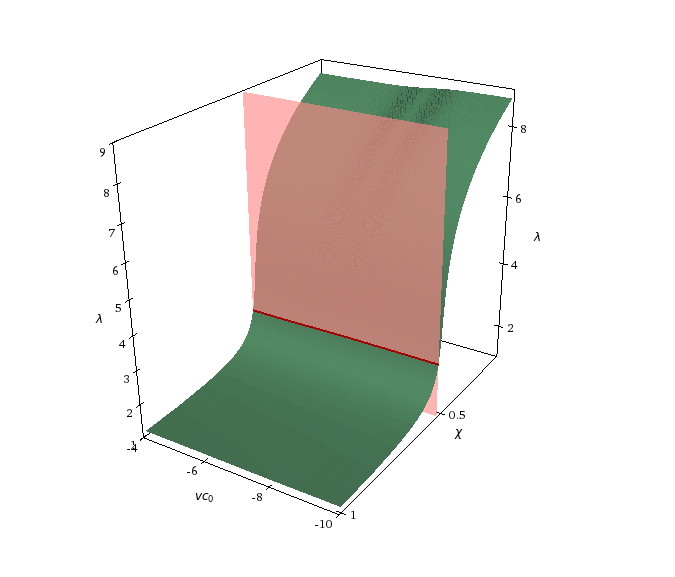
\includegraphics[scale=0.25]{images/manifold}
		\caption{}
	\end{subfigure}
	\hspace{-5mm}
	\begin{subfigure}{0.46\textwidth}
		\hspace{-3mm}
		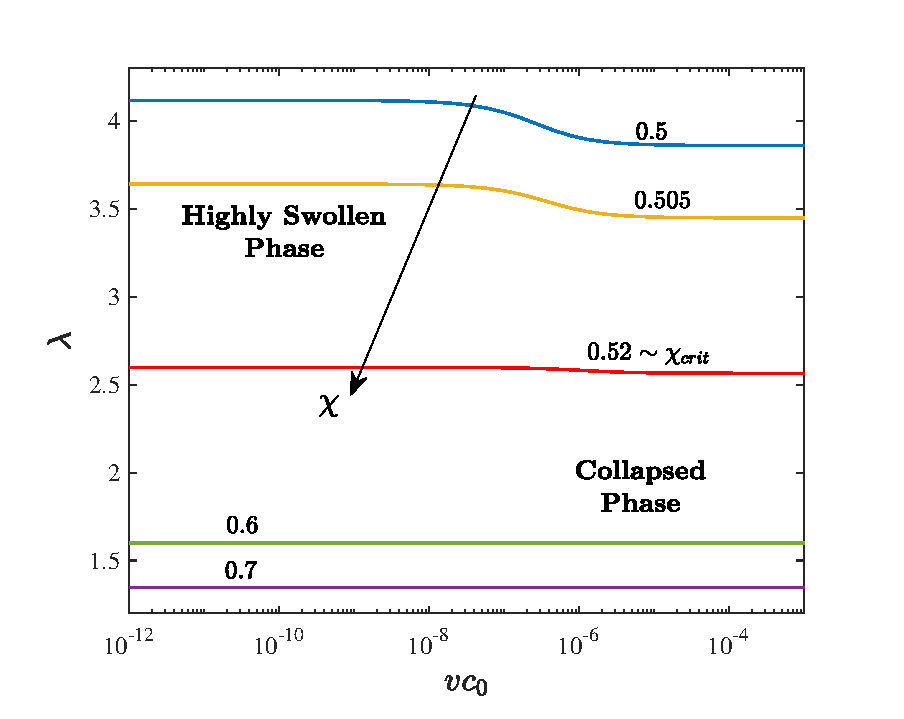
\includegraphics[scale=0.4]{images/free1}
		\caption{}
	\end{subfigure}
	\caption{Free Swelling: (a) Manifold implicitly defined by Equation~(\ref{eqF}) where $G^A_{eq}=10^3$ is fixed, while $c_0$ and $\chi$ are varied. On the vertical axis, we have plot $\lambda$ as defined by~(\ref{deffree}). In the red, it is highlighted the plane corresponding to $\chi=\chi_{crit}$ that split the parameter space into the region of high swelling and collapse for the material \cite{}.}
	\label{analysis}
\end{figure}

As the model are equivalent, we conclude that common unconstrained swelling experiments that test the equilibrium state are not sufficient to discern between the two, but can be useful to estimate some of the several parameter in the model. 



%\subsection{Models B.}
In this second case, given the symmetry of the problem, we have that, at equilibrium the deviatoric component of the stress tensor $\mathbb{T}$ vanishes. Combining this information with the boundary condition and solving the system~(\ref{sys1B})-(\ref{sys2B}) for its equilibrium, we obtain the same equations as for model A, while the pressure is now defined as:
\begin{equation}
p = \frac{\partial \psi_{vol}}{\partial J} .\label{presB}%= \frac{\kappa}{1+C_s v_s}.
\end{equation}

We follow two different approaches, in case $BA$, we derive the constitutive equation for $\psi_{vol}$, so that the model B and model A predict the same equilibrium behaviour, i.e. $p_A=p_{BA}$. Using Equations~(\ref{presA})-(\ref{presB}), and the constraint $\psi_{vol}(1)=0$, we obtain:
\begin{equation}
\frac{\partial \psi^{BA}_{vol}}{\partial J}= G^A_{eq} \frac{J^{2/3}-1}{J} \Longrightarrow \psi_{vol} = \frac{G^{BA}_{vol}}{2}\left[3(J^{2/3} -1) - 2\ln J\right],
\end{equation}
which is equivalent to using a Neo-Hookean model also for the volumetric spring with shear modulus $G^{BA}_{vol}$. In the second case, we instead consider a more commonly used constitutive model for volumetric deformation. Based on Equation~(\ref{psivol}), the pressure is given by:
\begin{equation}
p_{B} = \frac{\kappa}{1+C_s v_s}.
\end{equation}
Consequently, while Equation~(\ref{eqion}) still hold, we have that also the equilibrium condition~(\ref{eqF}) is now of the form:
\begin{equation}
\begin{aligned}
F_{B}(C_s; c_0,\chi,\kappa)=&\frac{1+C_sv_s+\chi}{(1+C_sv_s)^2}+\frac{\kappa v_s}{k_BT} \frac{1}{1+C_sv_s}+\ln \frac{C_sv_s}{1+C_sv_s}\\[1.5mm]
& +2c_0v_s-\sqrt{\left(\frac{z_fC_f}{C_s}\right)^2+4v_s^2c^2_0} =0 \label{eqFb}
\end{aligned}
\end{equation}
\subsection{Comparison of the Models.}

By construction, the model $A$ and $BA$ agrees. On the other hand, as illustrated in Figure~\ref{Exp1}(b), the discrepancy with model B depends on the real elastic properties of the material tested. In particular, the softer the tissue, the larger is the difference between the two. Looking at Figure~\ref{Exp1}(b), the major discrepancy is in the equilibrium behaviour at the two limits: $c_0$ small and $c_0$ large. 

\begin{figure}[h]
	\begin{subfigure}{0.6\textwidth}
		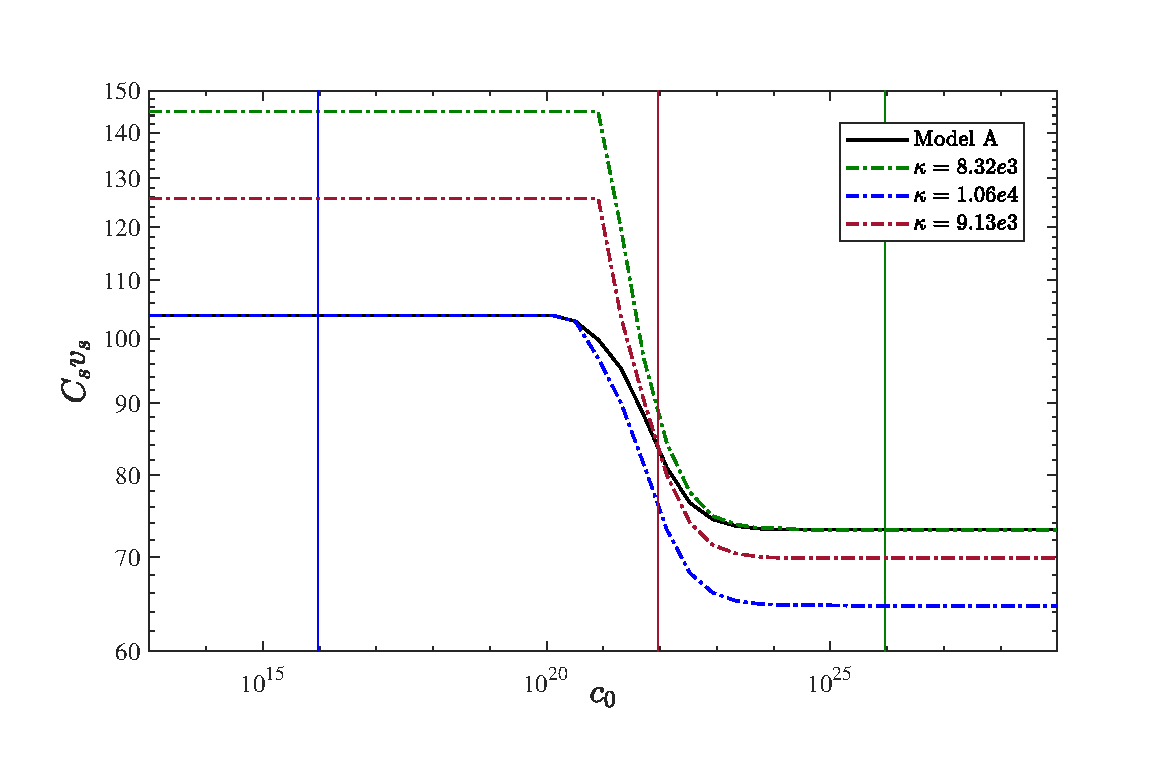
\includegraphics[scale=0.36]{images/freeswel1}
		\caption{$G^A_{eq}=5e3$}
	\end{subfigure}
	\begin{subfigure}{0.39\textwidth}
		\hspace{-8mm}
		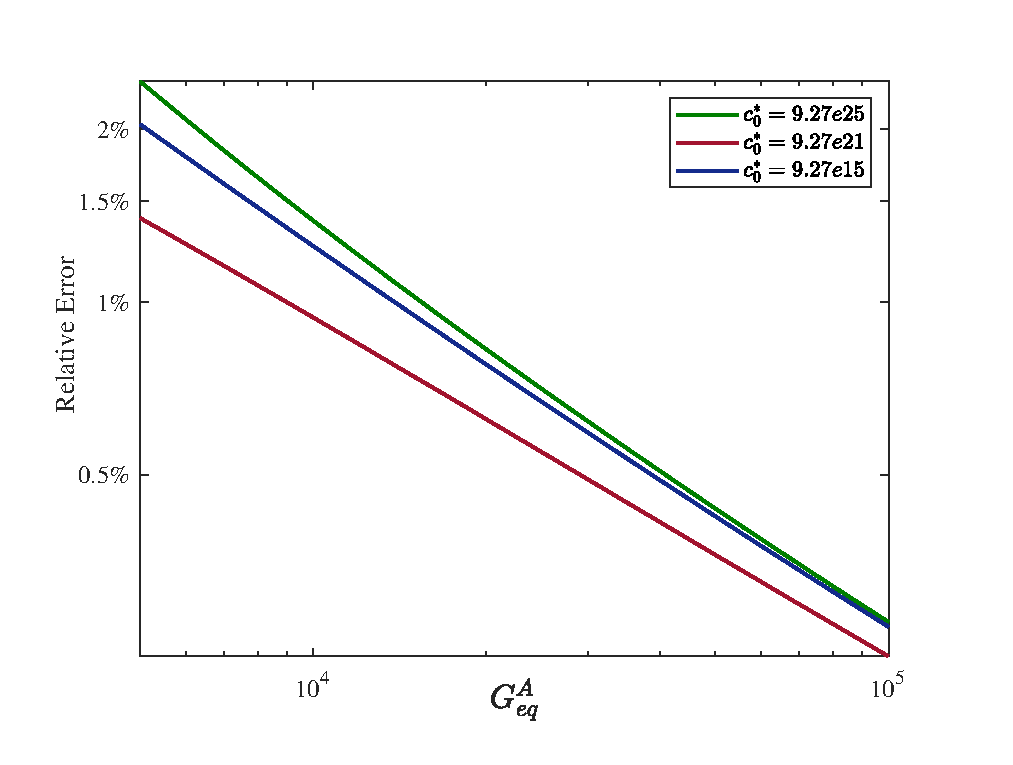
\includegraphics[scale=0.36]{images/freeswel2}
		\caption{}
	\end{subfigure}
	\vspace{3mm}
	\caption{Comparison of the prediction for the two models in a Free Swelling experiment. We consider as a reference Model A (ground truth). We fix the concentration $c^*_0$ of ions in the bath, we leave the matrix reach is steady state and we measure $C_s(c^*_0)$. Using Equations~(\ref{eqF})-(\ref{eqFb}) we have $\kappa(c^*_0)=G^A_{eq}((1+v_sC_s)^{2/3}-1)$. The same is repeated for three different salt concentration (each experiment correspond to a colour,see legend of Figure (b)). (a) 
		Comparison between Model A and Model B for the different estimated values $\kappa(c^*_0)$. (b) Relative error between the model as a function of the matrix stiffness $G_{eq}^A$. We note that the softer the matrix, the larger is the discrepancy between the two model. The choice of $c^*_0$ can also impact on the estimated error. Given the same mixing parameter $\chi$, the two models can not agree on the equilibrium behaviour for the two limits: $c_0$ small or $c_0$ large. Consequently the best choice would be choosing $c_0$ in the region of transition. Note that the shear modulus of the ECM is estimated to be of order $10^3-10^4$ \cite{Netti}.}
	\label{Exp1}
\end{figure}

If we consider instead the mixing parameter $\chi$ to be also unknown, then there is a set of parameter values for which the models predict the same equilibrium swelling fraction, see Figure \ref{freeA}. However, as illustrated in Figure \ref{freeB}, there are several order of magnitude of difference in the expected pressure inside the gel. Such discrepancy depend on the phase of the ECM. As discussed in \cite{}, polyelectrolytes can undergo a discontinuous phase transition between an highly swollen, i.e. $C_s>>1$, and a collapsed phase, i.e. $C_s\sim<1$. As shown in Figure \ref{freeC}, the state depends on the value of the mixing parameter $\chi$ and thus on the osmotic pressure $\Pi^n$ in the ECM. While the models agree in predicting the collapsed phase, i.e. small deformation, there is a great difference in the expected mixing properties in the case of large changes in the ECM volume. 

\begin{figure}[h]
	\begin{subfigure}{0.49\textwidth}
		\centering
		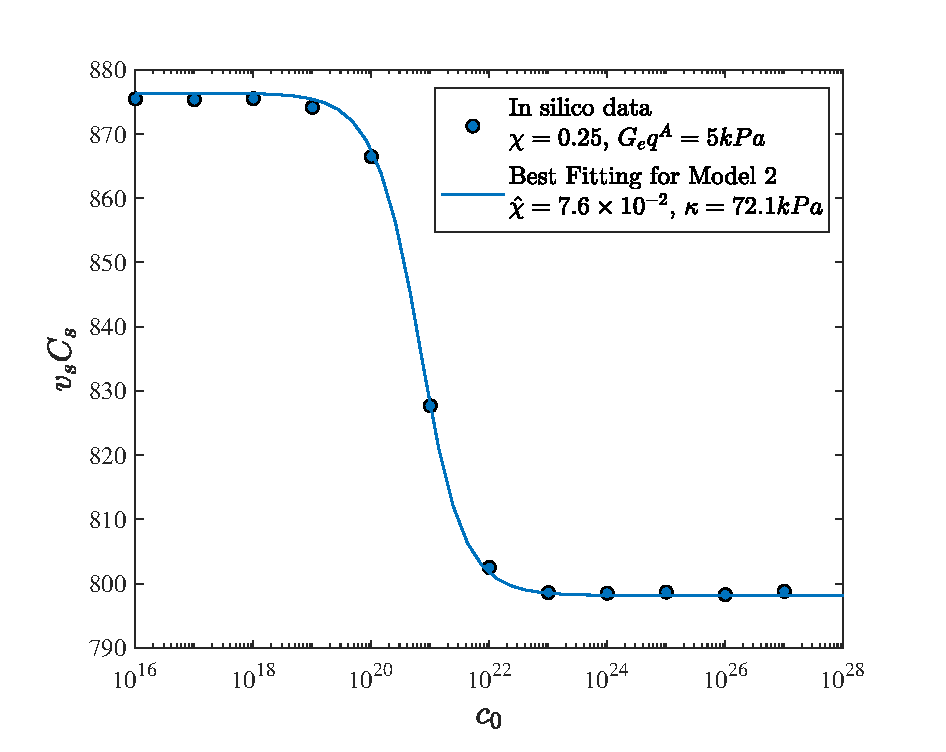
\includegraphics[scale=0.32]{images/chi2}
		\caption{}
		\label{freeA}
	\end{subfigure}	
	\begin{subfigure}{0.49\textwidth}
		\centering
		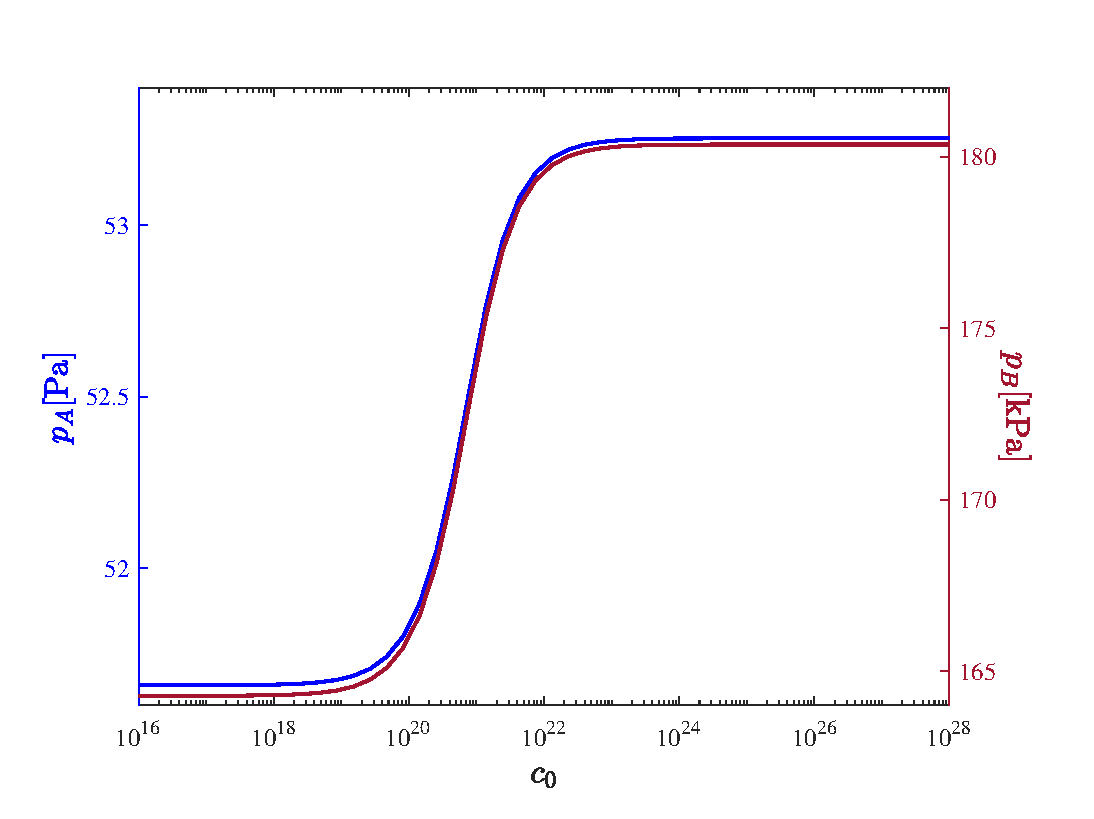
\includegraphics[scale=0.285]{images/chi3p}
		\caption{}
		\label{freeB}
	\end{subfigure}	
	
	\centering
	\begin{subfigure}{0.6\textwidth}
		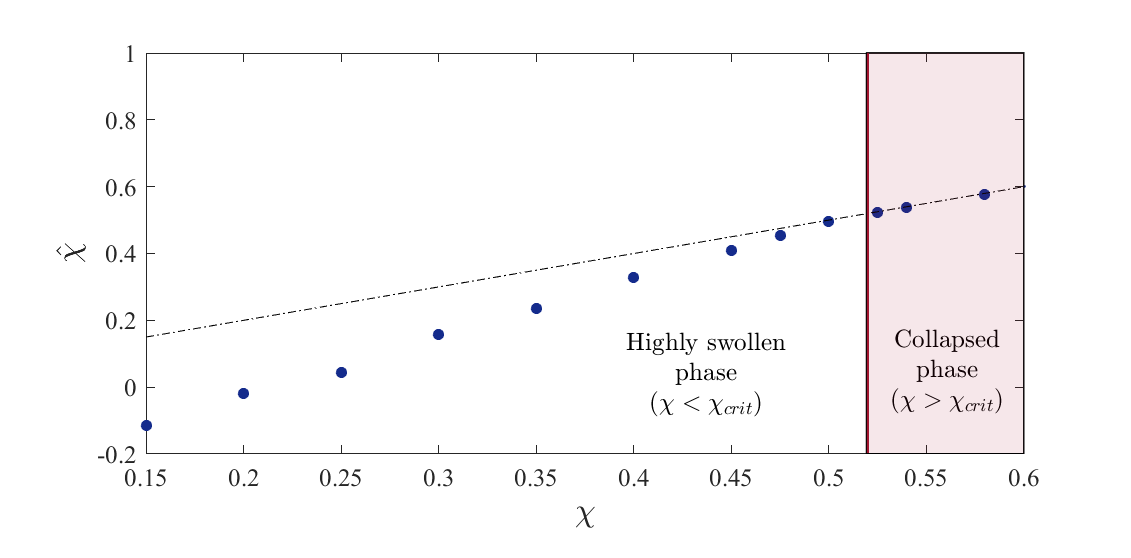
\includegraphics[scale=0.415]{images/chi1}
		\caption{}
		\label{freeC}
	\end{subfigure}
	\caption{Model Comparison 2: despite there is a set of parameters that would give rise to the same equilibrium behaviour this can drastically change the predicted mixing properties of the ECM. (a-b) Example of an \textit{in silico} experiment for $G^A_{eq}=5e2$: data are generated using model A and adding random noise. The fitting for model B is obtained using the non-linear least square method function in MATLAB, \texttt{fmincon}. (a) Predicted equilibrium concentration of water in the ECM; (b) Predicted mechanical pressure in the ECM from model A (blue) and model B (red). Despite capturing the same qualitative trend, the two differ of several order of magnitude. (c) Flory-Huggins parameter $\chi$ used in the \textit{in silico} experiment vs the one estimated fitting model B to the \textit{in silico} data $\hat{\chi}$; .}
	\label{figfree2}
\end{figure}

Based on our analysis, a simple unconstrained swelling experiment is informative only if, either $\chi$ is known or the pressure inside the ECM is known. However, when dealing with tissue, it is unlikely to be the case. Based on our current knowledge, there are no quantitative studies focusing on the value of $\chi$. Similarly, previous studies rely on mathematical models to estimate the pressure as experimentally measures can be challenging \cite{pressure,ecm1,ecm2}. 
\section{Confined Compression Test.}

\begin{figure}[h]
	\centering
	\def\svgwidth{0.89\linewidth}
	\input{latex/images/compression.pdf_tex}
	\vspace{2mm}
	\caption{Schematic representation of a compression test with a porous piston. A deformation is imposed in the $Z$ direction and the force necessary to maintain the deformation is recorded. }
\end{figure}

In this second example, we consider to perform on a swollen slice of ECM a compression test with the use of a porous platen,which allows the fluids to flow so to maintain the chemical equilibrium with the external bath \cite{Netti}. This allows to measure both the dynamical and equilibrium behaviour of the material by measuring the stress while imposing a known strain $\epsilon$. The corresponding deformation tensor is of the form:

\begin{equation}
\F=J_0^{1/3}\begin{bmatrix}
1 &0&0\\
0&1&0\\
0&0& \lambda_1
\end{bmatrix},
\label{F} 
\end{equation}
where $\lambda_1 = 1 - \epsilon$. 
\subsection{Model A}
As before, given the symmetries of the system, $\B_e$ is a diagonal matrix of the form:
\begin{equation}
\B_e=\begin{bmatrix}
b &0&0\\
0&b&0\\
0&0& b_1
\end{bmatrix}. 
\end{equation}
Again we are here interested in the equilibrium behaviour, for which Equations~(\ref{eqion}) still holds. Focusing on the contribution of spring B, studying the equilibriums of Equation~(\ref{Be}), we obtain that $b=b_1$. Since $\det \B_e= (\det \F)^2$, we conclude that:
\begin{equation}
b = J_0^{2/3}\lambda_1^{2/3}.
\end{equation}

Using the boundary condition, we can now compute the pressure and the equilibrium condition:
\begin{gather}
p = -\sigma + \frac{G^A_1}{J_0\lambda_1} (J^{2/3}_0\lambda_1^2-1)+\frac{G^A_2}{J_0\lambda_1} (J_0^{2/3} \lambda_1^{2/3}-1) \\
\begin{aligned}
\frac{\sigma v_s}{k_B T}=&\frac{J_0\lambda_1+\chi}{J_0^2\lambda^2_1}+\frac{G_1^Av_s}{k_BT} \frac{J_0^{2/3}\lambda^2_1-1}{J_0 \lambda_1}+\frac{G_2^Av_s}{k_BT} \frac{J_0^{2/3}\lambda^{2/3}_1-1}{J_0 \lambda_1}\\[1.5mm]
&+\ln \frac{J_0\lambda_1-1}{J_0\lambda_1} +2c_0v_s-\sqrt{\left(\frac{z_fC_fv_s}{J_0\lambda_1-1}\right)^2+4v_s^2c^2_0}\label{compA}
\end{aligned}
\end{gather}

\subsection{Models B.}
Based on Equation~(\ref{F}), we have that the tensors $\bar{\B}$ and $\bar{\B}_e$ are of the form:
\begin{equation}
\bar{\B}=\begin{bmatrix}
\lambda_1^{-2/3} &0&0\\
0&\lambda_1^{-2/3}&0\\
0&0& \lambda_1^{4/3}
\end{bmatrix}, \qquad
\bar{\B}_e=\begin{bmatrix}
\bar{b} &0&0\\
0&\bar{b}&0\\
0&0& \bar{b}_1
\end{bmatrix}
\end{equation}

As for the model A, at equilibrium we have that $\bar{b}=\bar{b}_1$. However, in this case, we have that $\det \bar{B}_e=1$ so that $\bar{b}=1$ so that the second spring does not contribute to the stress. Using the boundary condition, in the case of model $BA$ we obtain:
\begin{gather}
\displaystyle 
p_{BA} = -\sigma + \frac{G^A_{eq}}{J_0\lambda_1}(J_0^{2/3}\lambda_1^{2/3}-1)+\dfrac{2G^B_1}{3J_0\lambda_1^{5/3}} (\lambda_1^2-1) \\
\begin{aligned}
\frac{\sigma v_s}{k_B T}=&\dfrac{J_0\lambda_1+\chi}{J_0^2\lambda^2_1}+\frac{2G_1^Bv_s}{3k_BT} \dfrac{\lambda^2_1-1}{J_0 \lambda_1^{5/3}}+\frac{G^A_{eq}v_s}{k_BT}\frac{J_0^{2/3}\lambda_1^{2/3}-1}{J_0\lambda_1}\\[1.5mm]
& +\ln \frac{J_0\lambda_1-1}{J_0\lambda_1}+2c_0v_s-\sqrt{\left(\frac{z_fC_fv_s}{J_0\lambda_1-1}\right)^2+4v_s^2c^2_0}.\label{compAB}
\end{aligned}
\end{gather}

Unlike the case of unconstrained swelling, we now have that the model $A$ and $BA$ are substantially different, so that there is no choice of the parameter that would predict the same stress-strain behaviour. This highlights how, the choice of a particular decomposition of the deformation gradient $\F$ correspond to a modelling decision on the constitutive properties of the material under study.  
while for model $B$, the equilibrium conditions are:
\begin{gather}
\displaystyle 
p_B = -\sigma + \frac{\kappa}{J_0\lambda_1}+\dfrac{2G^B_1}{3J_0\lambda_1^{5/3}} (\lambda_1^2-1) \\
\begin{aligned}
\frac{\sigma v_s}{k_B T}=&\dfrac{J_0\lambda_1+\chi}{J_0^2\lambda^2_1}+\frac{2G_1^Bv_s}{3k_BT} \dfrac{\lambda^2_1-1}{J_0 \lambda_1^{5/3}}+\frac{\kappa v_s}{k_BT} \frac{1}{J_0 \lambda_1}+\ln \frac{J_0\lambda_1-1}{J_0\lambda_1}\\[1.5mm]
& +2c_0v_s-\sqrt{\left(\frac{z_fC_fv_s}{J_0\lambda_1-1}\right)^2+4v_s^2c^2_0}.
\end{aligned}
\end{gather}

\subsection{Model Comparison.}
We first focus on comparing the model $A$ and $AB$, assuming that the parameter $\chi$ is fixed and that $G^{AB}_{vol}=G^A_{eq}$, so that the equilibrium volume $J_0$ is the same for both models. If we now take the difference between Equations~(\ref{compA}) and (\ref{compAB}), we obtain that the difference in the compression stress $\delta \sigma= \sigma_{BA}-\sigma_{A}$ is:
\begin{equation}
\delta \sigma = \frac{2 G_1^{AB}}{3} \frac{\lambda_1^2-1}{J_0\lambda_1^{5/3}} - \frac{G_1^A}{J_0^{1/3}}(\lambda_1-\lambda_1^{-1/3}).\label{err}
\end{equation}
Looking at the above equation it appears clearly that there is no constant value of $G^{AB}_1$ for which the difference $\delta \sigma$ is identically zero. If we impose that for small deformation, i.e. $\lambda_1\rightarrow 1$, the two models agree at the second order:
\begin{equation}
\delta \sigma=0, \qquad \frac{\d \delta \sigma}{\d \lambda_1}=0 \quad\Rightarrow \quad G_1^{AB} = J_0^{2/3}G_1^A.
\end{equation}
Under such condition we can rewrite the Equation~(\ref{err}) as:
\begin{equation}
\delta \sigma(\lambda_1;G^A_1,J_0) = \frac{G_1^A}{J^{1/3}_0\lambda_1^{5/3}} \left(\frac{2}{3}\lambda^2_1-\frac{2}{3}-\lambda_1^{5/3}+\lambda_1^{4/3}\right), 
\end{equation}
which is unbounded for large deformation, i.e. $\lambda_1\Rightarrow0$.
%We here consider another standardd
\begin{figure}
	\hspace{-8mm}
	\begin{subfigure}{0.62\textwidth}
		\hspace{6mm}
		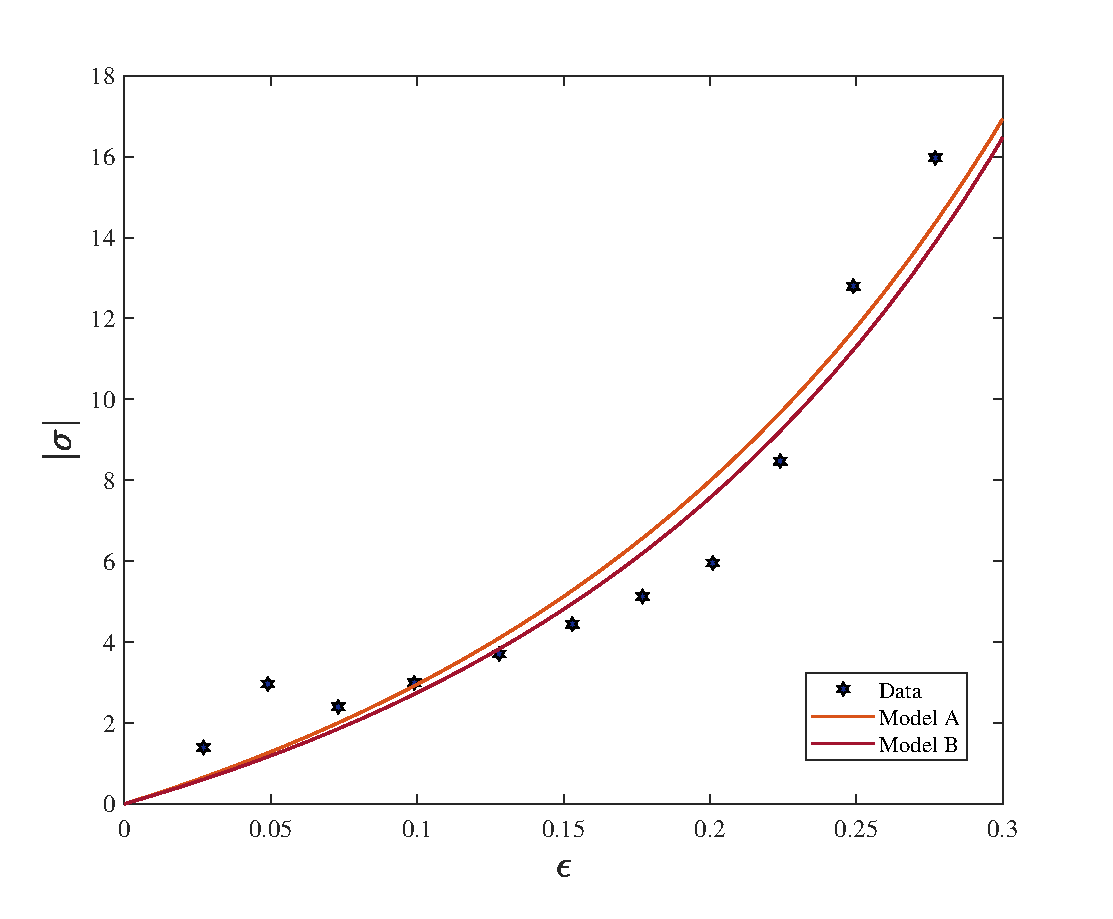
\includegraphics[scale=0.35]{images/compression.eps}
		\caption{Fitted Model}
		\label{fit}
	\end{subfigure}
	\begin{subtable}{0.375\textwidth}
			\begin{tabular}{c | c ||c| c }		
				\hline\addlinespace[2pt]
				 \multicolumn{2}{c||}{Model A} &  \multicolumn{2}{c}{Model B}\\[0.5mm]
				\hline\addlinespace[2pt]
				$\quad \chi\quad$ & $\quad0.498\quad$ &$\quad \chi\quad$&$\quad0.523\quad$\\[0.5mm]
				$G^A_1$ & 18.9 kPa&$\kappa$& 0.83 kPa\\[0.5mm]
				$G^A_2$ & 5.3 Pa&$G^B_1$& 55.1 kPa\\[0.5mm]
				$J_0$ & $20.7$&  $J_0$&$14.8$\\[0.5mm]
				\hline\addlinespace[2pt]
				\multicolumn{4}{c}{Model BA}\\[0.5mm]
				\hline\addlinespace[2pt]
				\multicolumn{2}{c|}{$\chi$} & \multicolumn{2}{c}{0.524}  \\
				\multicolumn{2}{c|}{$G_{vol}$} & \multicolumn{2}{c}{75 Pa}  \\
	            \multicolumn{2}{c|}{$G^{BA}_{1}$} & \multicolumn{2}{c}{55.1 kPa} \\
				\multicolumn{2}{c|}{$J_0$} & 	\multicolumn{2}{c}{ 14.8}\\
				\hline
			\end{tabular}
		\caption{Estimated Parameters}
		\label{param}
	\end{subtable}
\caption{Comparison of the two model in fitting real experimental data from \cite{Netti}.}		
\end{figure}

As shown in Figure \ref{fit}, both models are able to capture the qualitative behaviour of the data. However, as shown by the parameters in Table \ref{param}, there are quantitative differences. In particular, there are order of magnitude of difference in the estimated pressure $p$. If we look at its value for zero-strain, i.e. $\lambda_1=1$, we obtain: 
\begin{gather}
p_A = \frac{G^A_1+G^A_2}{J_0}(J_0^{2/3}-1) = \frac{24.2 \text{ kPa}}{20.7}(20.7^{2/3}-1) = 7.64 \text{ kPa},\\
p_{BA} = \frac{G_vol}{J_0}(J_0^{2/3}-1) = \frac{0.075 \text{ kPa}}{14.8}(14.8^{2/3}-1) = 25.5 \text{ Pa}\\
p_B = \frac{\kappa}{J_0} = \frac{0.83 \text{ kPa}}{14.8} = 56.08 \text{ Pa}
\end{gather}

When designing synthetic ECM, the tuning of the internal pressure cells in a culture are exposed to is of large importance. As mentioned in the introduction, cells are sensitive to pressure and their response can greatly change depending on this stimulus. Consequently, depending on the model chosen, the

\section{Confined Compression Test.}
\label{excomp}
A second common test conducted on soft material is confined compression. As illustrated in Figure \ref{confcomp}, a porous plate is used so that the fluid is free to flow and the chemical equilibrium with the external bath is restored after the transient relaxation phase. After gradual compression of the tissue, the system is allowed to relax while the strain $\epsilon$ is maintained constant \cite{Netti}. We here interested in the equilibrium, i.e. relaxed, behaviour of the sample, which is described by a stress-strain curve (see Figure \ref{fit} as an example). 

\begin{figure}[h]
	\centering
	\def\svgwidth{0.89\linewidth}
	\input{latex/images/compression.pdf_tex}
	\vspace{2mm}
	\caption{Schematic representation of a compression test with a porous piston. A deformation is imposed in the $Z$ direction and the force necessary to maintain the deformation is recorded. }
	\label{confcomp}
\end{figure}

As we consider a swollen slice of tissue compressed in the $Z$ direction, the deformation $\F$ from the dry to the current state has the form:

\begin{equation}
\F=J_0^{1/3}\begin{bmatrix}
1 &0&0\\
0&1&0\\
0&0& \lambda_1
\end{bmatrix},
\label{F} 
\end{equation}
where $\lambda_1 = 1 - \epsilon$ and $J_0$ defines the initial swollen state. 

As the problem is one-dimensional, we can reduce the number of unknowns. We define $u=\mathbf{u}\,\cdot\,\mathbf{e}_Z$, $T_{zz}= \mathbf{e}_Z \mathbb{T}\mathbf{e}_Z$ and $J_m=\mathbf{J}_m\,\cdot \,\mathbf{e}_Z$, the component of the displacement, deformation tensor and fluxes in the $Z$ direction. Assuming the slice to have an initial height $H_0$, proper boundary conditions need to be assigned at the two edges $Z=0$ and $Z=H_0$:
\begin{eqnarray}
\left[\mu_s\right]^+_-=\left[\mu_+\right]^+_-=\left[\mu_-\right]^+_-=0, \quad \left[T_{zz}\right]^+_-=0, &\qquad& Z=H_0\,,\\
J_m = u = 0, &\qquad& Z=0\, ,\\
\frac{\d \Phi}{\d Z}=0 &\qquad& Z=0,H_0\,.
\end{eqnarray}

At equilibrium, the conditions~1 and 2 listed in Section \ref{free} still hold. On the other hand, due to the external force $\mathbf{F}= -F_z \mathbf{e}_z$ which is exerted on the plate of area $A$, condition 3 now reads:

\begin{equation}
T_{zz}=\sigma = -\frac{F_z}{A}.
\end{equation} 

\subsection{Model Comparison.}
\label{data}
Starting from model A, given the symmetries of the problem, $\B_e$ is a diagonal matrix of the form:
\begin{equation}
\B_e=\begin{bmatrix}
b &0&0\\
0&b&0\\
0&0& b_1
\end{bmatrix}. 
\end{equation}
If we now study the fixed point of Equation~(\ref{Be}), we obtain that $b=b_1=J_0^{2/3}\lambda_1^{2/3}$ as $\det \B_e= (\det \F)^2$.

Focusing on model B instead, the tensors $\bar{\B}$ and $\bar{\B}_e$ are now of the form:
\begin{equation}
\bar{\B}=\begin{bmatrix}
\lambda_1^{-2/3} &0&0\\
0&\lambda_1^{-2/3}&0\\
0&0& \lambda_1^{4/3}
\end{bmatrix}, \qquad
\bar{\B}_e=\begin{bmatrix}
\bar{b} &0&0\\
0&\bar{b}&0\\
0&0& \bar{b}_1
\end{bmatrix}
\end{equation}
with the $\bar{b}=\bar{b}_1=1$ at equilibrium so that the spring $2$ does not contribute to the stress. Substituting the equilibrium conditions into the state equations for the two models (see Table \ref{summary}) yields to:
\begin{gather}
p = \begin{cases}
\displaystyle
-\sigma + \frac{G^A_1}{J_0\lambda_1} (J^{2/3}_0\lambda_1^2-1)+\frac{G^A_2}{J_0\lambda_1} (J_0^{2/3} \lambda_1^{2/3}-1) &\quad \text{MODEL A} \\[10pt]
-\sigma + \dfrac{G_{vol}}{J_0\lambda_1}(J_0^{2/3}\lambda_1^{2/3}-1)+\dfrac{2G^B_1}{3J_0\lambda_1^{5/3}} (\lambda_1^2-1) &\quad \text{MODEL B}
\end{cases}\\[10pt]
\begin{aligned}
\frac{\sigma v_s}{k_B T}=\frac{J_0\lambda_1+\chi}{J_0^2\lambda^2_1}+\frac{pv_s}{k_B T}+&\ln \frac{J_0\lambda_1-1}{J_0\lambda_1} +2c_0v_s\\
-\ &\sqrt{\left(\frac{z_fC_fv_s}{J_0\lambda_1-1}\right)^2+4v_s^2c^2_0}
\end{aligned}\label{compA}
\end{gather}

Unlike for unconstrained swelling, we note that model $A$ and $B$ are now substantially different, as there is no choice of parameter values for which the two are equivalent for any value of $\lambda_1$. 

Following the work of Xue et al~\cite{ecm2}, we test our models on the data collected by Netti et~al. \cite{Netti} on HSTS 26T sarcoma slices. Despite our model being built to describe decellularized ECM, cells can be included in the model simply as part of the solid phase \cite{ecm2}. As we are interested in the tissue scale, this is a good approximation. However, as suggested also by Xue et~al.\cite{ecm2}, more accurate models also incorporate the cellular activities. However, this goes beyond the purpose of our study.

\begin{figure}[h]
	\hspace{-8mm}
	\begin{subfigure}{0.62\textwidth}
		\hspace{2mm}
		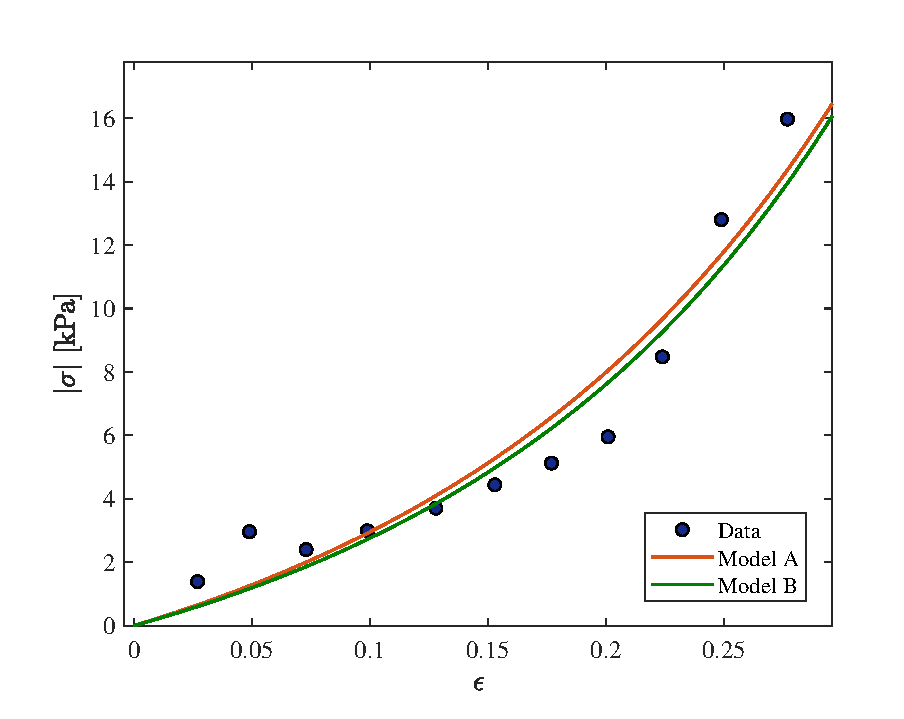
\includegraphics[scale=0.42]{images/compression2.eps}
		\caption{Fitted Model}
		\label{fit}
	\end{subfigure}
	\begin{subtable}{0.375\textwidth}
		\begin{tabular}{c | c ||c| c }		
			\hline\addlinespace[2pt]
			\multicolumn{2}{c||}{Model A} &  \multicolumn{2}{c}{Model B}\\[0.5mm]
			\hline\addlinespace[2pt]
			$\quad \chi\quad$ & $\quad0.498\quad$ &$\quad \chi\quad$&$\quad0.524\quad$\\[0.5mm]
			$G^A_1$ & 18.9 kPa&$G_{vol}$&75 Pa\\[0.5mm]
			$G^A_2$ & 5.3 Pa&$G^{B}_{1}$& 55.1 kPa\\[0.5mm]
			$J_0$ & $20.7$&  $J_0$&$14.8$\\[0.5mm]
			\hline
		\end{tabular}
		\caption{Estimated Parameters}
		\label{param}
	\end{subtable}
	\caption{Comparison of the two models in fitting real experimental data from \cite{Netti}.}		
\end{figure}

Together with the stress-strain curve from the compression test, Netti et~al. measure also the tissue composition, so that $C_f$ is known (see Table \ref{Tab1}). The other parameters listed in Table \ref{Tab1} have been taken from the literature. Consequently the set of unknown parameters is $\left\{\chi, G^A_1, G^A_2\right\}$ and $\left\{\chi, G_{vol}, G^B_1\right\}$ for models A and B respectively. These are estimated fitting Equation~(\ref{compA}) to the data, using the \texttt{fmincon} function in MATLAB, which implements the non-linear least squares method\footnote{the result as been optimized starting from different initial condition, so to explore a larger part of the parameter space}.

As shown in Figure \ref{fit}, both models are able to capture the qualitative behaviour of the data. However they largely disagree in their quantitative predictions, see Table \ref{param}. Let us for example compute the initial pressures in the tissue slice, i.e. $p$ at $\lambda_1=1$:  
\begin{gather}
p_A = \frac{G^A_1+G^A_2}{J_0}(J_0^{2/3}-1) = \frac{24.2 \text{ kPa}}{20.7}(20.7^{2/3}-1) = 7.64 \text{ kPa},\\
p_B = \frac{G_{vol}}{J_0}(J_0^{2/3}-1) = \frac{0.075 \text{ kPa}}{14.8}(14.8^{2/3}-1) = 25.5 \text{ Pa},
\end{gather}
then the two differ of several order of magnitude. Consequently, the models give a completely different estimation of the pressure cells in the tissue are exposed to. As hydrostatic pressure affect cells behaviour \cite{viscocell}, based on which model is considered, we could end up with completely different conclusion on the mechano-sensitivity of cells.
\begin{figure}[h!]
	\begin{subfigure}{0.49\textwidth}
		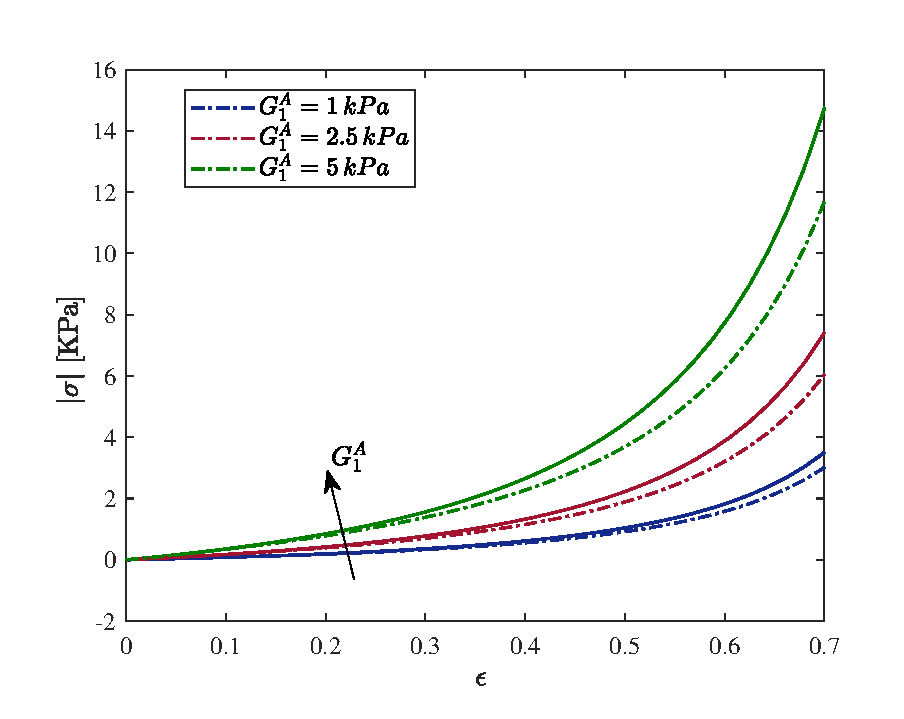
\includegraphics[scale=0.4]{images/comp1}
		\caption{}
	\end{subfigure}
	\begin{subfigure}{0.49\textwidth}
		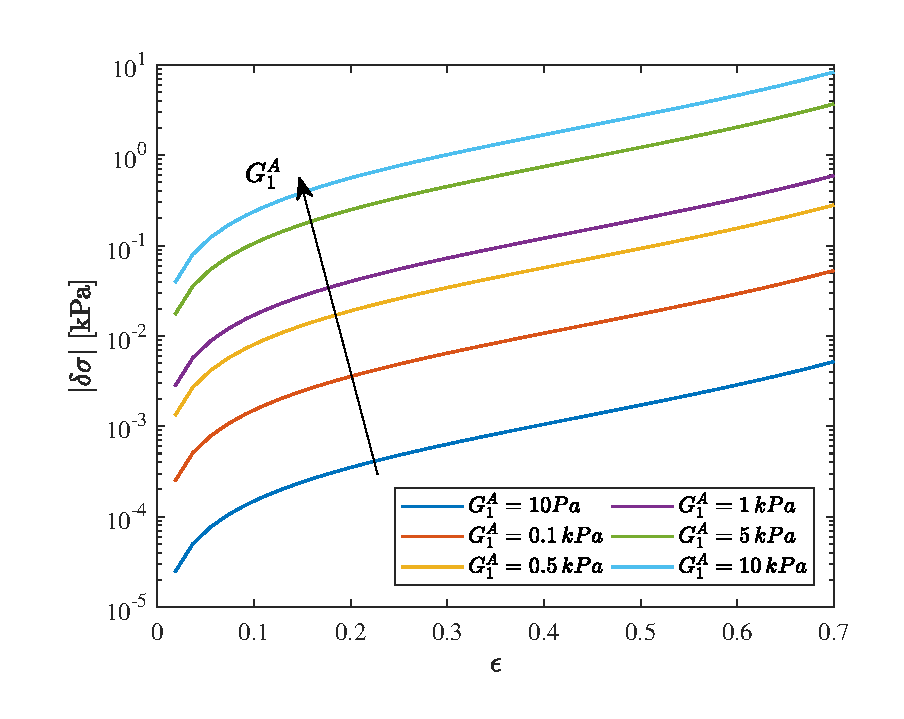
\includegraphics[scale=0.4]{images/comp2}
		\caption{}
	\end{subfigure}
	
	\begin{subfigure}{0.49\textwidth}
		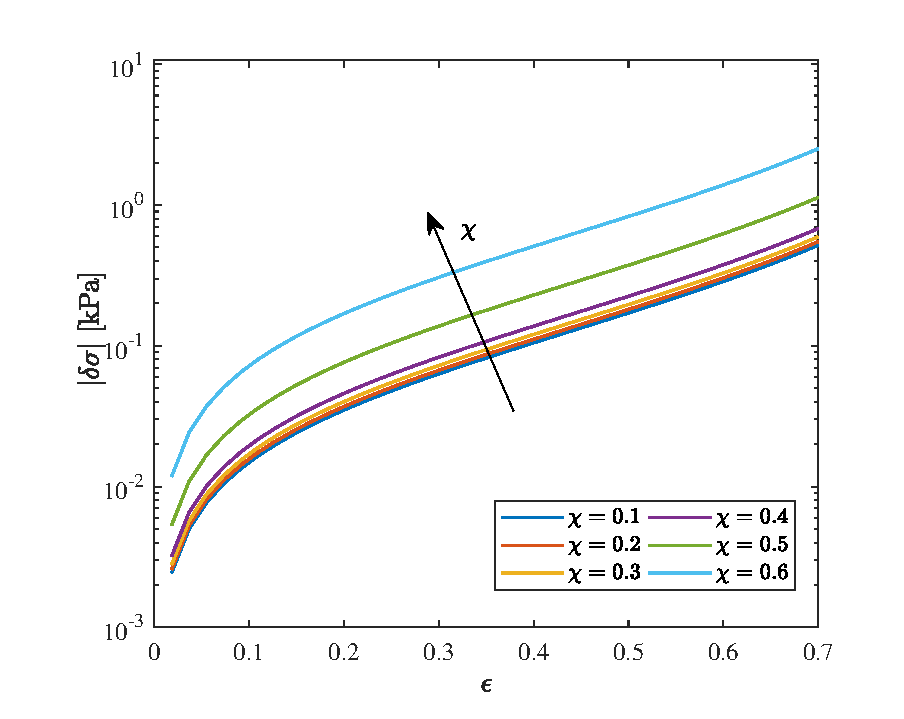
\includegraphics[scale=0.4]{images/comp3}
		\caption{}
	\end{subfigure}
	\begin{subfigure}{0.49\textwidth}
		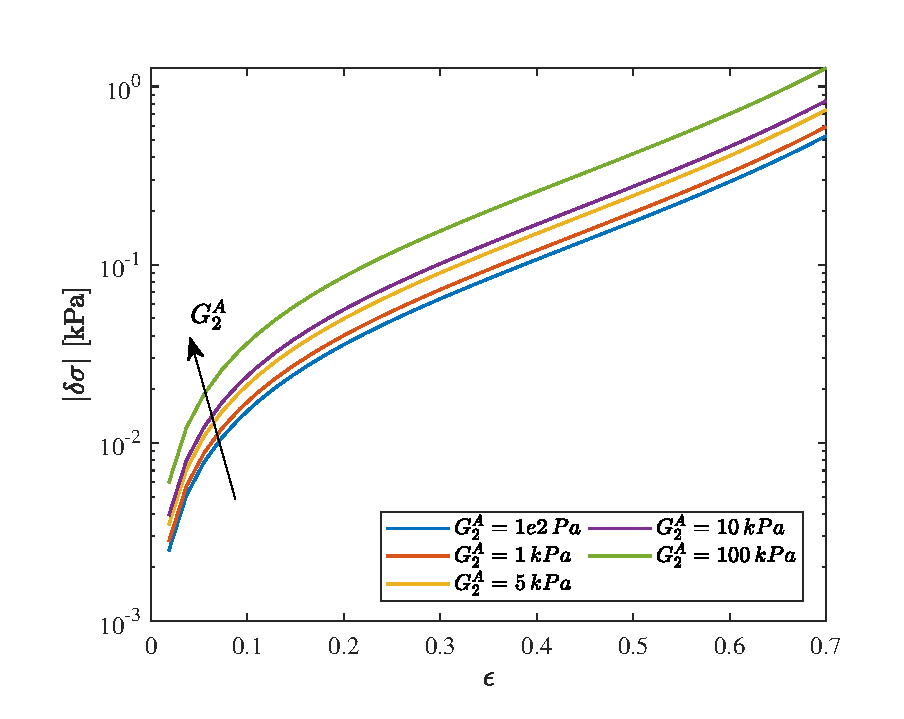
\includegraphics[scale=0.4]{images/comp4}
		\caption{}
	\end{subfigure}
	\caption{Sensitivity Analysis. As expected the mismatch between the two models grows with the strain: (a) Comparison of stress-strain curve predicted by model A (dotted line) and model B (full line) for different values of the parameter $G^A_1$; (b) as $G_1^A$ increases so does the discrepancy $\delta\sigma$; (c) $\delta\sigma$ is also particularly sensitive to changes in the mixing parameter $\chi$, in particular we see that there is a relevant jump when the ECM is in the \textit{collapsed} phase; (d) on the other hand, only large changes in $G^A_2$ have a relevant impact on $\delta\sigma$.}
	\label{comp3}
\end{figure}

Looking at the Table  \ref{param}, we note that $G_{vol}\neq G^A_{1}+G^A_2$, so that, the two estimated models would disagree also in the case of free-swelling. Based on the result from Section \ref{free}, we propose that a two-step protocols which combines free-swelling and compression test can be more informative to identify the material properties. To reproduce this setting \textit{in silico}, we compare again models $A$ and $B$ simulating a compression experiment. This time however we assume that the parameters $\chi$ and $G_{vol}=G^A_{eq}$ are fixed, as if they have been previously estimated by unconstrained swelling experiment. If we now take the difference between the compression stress predicted by Equation~(\ref{compA}) for the two models, i.e. $\delta \sigma= \sigma_{B}-\sigma_{A}$, we obtain:
\begin{equation}
\delta \sigma = \frac{2 G_1^{B}}{3} \frac{\lambda_1^2-1}{J_0\lambda_1^{5/3}} - \frac{G_1^A}{J_0^{1/3}}(\lambda_1-\lambda_1^{-1/3}).\label{err}
\end{equation}
For the purpose of our analysis, we impose the two models to agree at the second order in the regime of small deformation. This translates in the conditions $\lambda_1\rightarrow 1$:
\begin{equation}
\left.\delta \sigma\right|_{\lambda_1=1}=0 \qquad \left.\frac{\d \delta \sigma}{\d \lambda_1}\right|_{\lambda_1=1}=0 \quad\Rightarrow \quad G_1^{B} = J_0^{2/3}G_1^A.\label{temp14}
\end{equation}
Under such conditions we can rewrite Equation~(\ref{err}) as:
\begin{equation}
\delta \sigma(\lambda_1;G^A_1,J_0) = \frac{G_1^A}{J^{1/3}_0\lambda_1^{5/3}} \left(\frac{2}{3}\lambda^2_1-\frac{2}{3}-\lambda_1^{5/3}+\lambda_1^{4/3}\right), 
\end{equation}
where $J_0$ is defined by Equation~(\ref{eqF}). As shown in Figure \ref{comp3}, $\delta \sigma$ is an increasing function of $\epsilon$ as the two model appear to diverge exponentially as $\epsilon \rightarrow 0 $. Consequently, in the large-deformation regime we should be able to distinguish between the two models. Let us consider the case in which $\chi$ and $G_{vol}$ are estimated by free-swelling experiment as in Figure~(\ref{param}). Using Equation~(\ref{temp14}) and the condition $G_{vol}=G^A_{eq}$, we would have that $G^A_2<0$, which is not physically admissible. This is to highlight how, having information about free and constraint swelling can be informative in identifying the proper model. 

We could not find data from the literature for both swelling and compression tests on tissues, so that we can not yet conclude whether both, one or none of the models effectively describe soft tissue. This will require further experimental testing. With this aim, we have also performed a sensitivity analysis on the model parameters. As illustrated in Figure~(\ref{comp3}), $\chi$ and $G_1^A$ are the parameters that have the more impact on $\delta\sigma$. While $G_1^A$ depends only on the properties of the material, $\chi$ can be tuned by changing the temperature $T$ so to optimise the experimental condition. 


%We here consider another standardd


\newpage
\appendix
\section{Glossary of Variables and Parameters in the Model.}
\begin{table}[h!]
\begin{tabular}{c  l}
	$\psi\qquad $ & Helmholtz free energy per unit volume in the initial configuration,\\
	$\mathbf{u}\qquad$ & Displacement vector,\\
	$\F\qquad$ & Deformation gradient tensor $\F=\mathbb{I}-\nabla_0\mathbf{u}$,\\
	$C_f\qquad$ & Concentration of fix charges in the network,\\
	$z_f\qquad$ & Charge of a GAG chain,\\
	$v_m\qquad$ & Characteristic molecular volume of the species $m$,\\
	$\mathbf{u}\qquad$ & Displacement vector,\\
	$\F\qquad$ & Deformation gradient tensor $\F=\mathbb{I}-\nabla_0\mathbf{u}$,\\	
	$\mathbb{C}\qquad$ & Right Cauchy-Green Tensor $\mathbb{C}=\F^T\F$,\\
	$\mathbb{B}\qquad$ & Left Cauchy-Green Tensor $\mathbb{B}=\F\F^T$,\\
	$\LL\qquad$ & Velocity Gradient Tensor $\LL=\dot{\F}\F^{-1}$,\\
	$J\qquad$ & Determinant of the deformation gradient tensor $J=\det \F$,\\
	$\eta^A\qquad $ & Viscosity of the collagen network in model A,\\
	$G^A_1\qquad$ & Shear modulus related to spring $1$ in model A\\
	$G^A_2\qquad$ & Shear modulus related to spring $2$ in model A\\
	$G^B_1\qquad$ & Shear modulus related to spring $1$ in model B\\
	$G^B_2\qquad$ & Shear modulus related to spring $2$ in model B\\
	$\eta^B\qquad$ & Viscosity of the collagen network in model A,\\
	$\tau_R\qquad$ & Viscous relaxation time of the collagen network,\\
	$D^0_i\qquad$ & Diffusion coefficient for the $i$-th solute species when in pure solvent (interstitial fluid),\\
	$D_i\qquad$ & Diffusion coefficient for the $i$-th solute species in ECM,\\
	$K\qquad$ &  Hydraulic permeability of the ECM to the interstitial fluid (solvent+solute),\\
	$k\qquad$ &  Hydraulic  permeability  to  pure  solvent (water),\\
	$\kappa\qquad$ & Bulk modulus\\
	$\mathbb{T}^{Kort}\quad$ & Korteweg stress due to the ideal interface\\
	$\mathbb{T}^{Max}\quad$ & Maxwell stress due to the electric displacement\\
	$k_B\qquad$ & Boltzmann constant\\
	$T\qquad$ & Absolute Temperature \\
	$\text{DEV}\left[\cdot\right]\quad$ & Deviatoric part of the tensor $\text{DEV}\left[\cdot\right] = \cdot-1/3\, \text{tr}(\cdot)$
\end{tabular}	
\end{table}
%\section{f}
%\begin{gather}
%\boldsymbol{\xi} = \frac{\partial \psi}{\partial \nabla_0 C_s},\\
%\mu_s = p v -\nabla_0 \cdot \boldsymbol{\xi} + \frac{\partial \psi}{\partial C_s},\\
%\mu_i =  e\Phi z_i +\frac{\partial \psi}{\partial C_i},\hspace{5mm} i=1,\ldots,N ,\\
%\mathbf{E} = \frac{\partial \psi}{\partial \mathbf{H}} ,\label{ele}\\
%\mathbb{S} = -p J \F^{-T} + \frac{\partial \psi}{\partial \F}+ \frac{\partial \psi}{\partial\F_e}\F_v^{-1}\, ,\\
%\zeta_m =-T^{-1} \nabla_0 \,\mu_m,\\
%\zeta_v = T^{-1} \F_e^T\frac{\partial \psi}{\partial \F_e}.
%\end{gather}
\section{}
\begin{eqnarray}
\boldsymbol{\xi}&=&\frac{\partial \psi}{\partial \nabla_0 C}=,\\[2mm]
\mu &=& \frac{\partial \psi}{\partial C} - \nabla_0\cdot\boldsymbol{\xi}+ p v,\\[2mm]
\mathbb{S} &=&  \dfrac{\partial \psi}{\partial \F} + \dfrac{\partial \psi}{\partial \F_e}\F_v^{-T}- p J \F^{-T}
\end{eqnarray}

\section{Energy Dissipation.}
\label{apenergy}
Combining Equation~(\ref{vflow1}) and (\ref{vflow2}), and imposing that condition~(\ref{Jv}) is satisfied, we can characterise the viscous flow by the following relation:
\begin{equation}
\LL_v = L_{vv}T^{-1}\left[\F_e^T\frac{\partial \psi}{\partial \F_e}-p_v\mathbb{I}\right] \stackrel{(\ast)}{=} \frac{G^A_2}{\eta^A}\text{DEV}\left[\mathbb{C}_e\right] ,\label{Lv1}
\end{equation}
where $\eta^A$ represent the viscosity of the material and the equality $(\ast)$ follows from Equation~(\ref{temp4}):
\begin{equation}
\eta^A tr(\LL_v)= tr\left(\F_e^T\frac{\partial \psi}{\partial \F_e}\right) -  3 p_v=0 \Longrightarrow  p_v = \frac{tr\left(\F_e^T\frac{\partial \psi}{\partial \F_e}\right)}{3}.
\end{equation}
Using Equation~(\ref{hyp}), we obtain:
\begin{equation}
\LL_v = \frac{G^A_2 }{\eta^A}\text{DEV}[\mathbb{C}_e] = \frac{\text{DEV}[\mathbb{C}_e]}{2\tau_R}.\label{apBe}
\end{equation}

If we now consider the left elastic Cauchy Green tensor $\mathbb{B}_e=\F_e \F^T_e$, we can relate its time derivative to $\LL_v$:
\begin{equation}
\begin{aligned}
\dot{\mathbb{B}}_e &= \LL \mathbb{B}_e + \mathbb{B}_e \LL^T - 2 \F_e d_v \F_e^{T} \\
&= \LL\mathbb{B}_e + \mathbb{B}_e \LL^T - \frac{1}{\tau_R} \F_e\left[\mathbb{C}_e-\frac{1}{3}tr(\mathbb{B}_e)\mathbb{I}\right]\F_e^T\\
&= \LL\mathbb{B}_e + \mathbb{B}_e \LL^T - \frac{1}{\tau_R} \,\mathbb{B}_e\underbrace{\left[\mathbb{B}_e-\frac{1}{3}tr(\mathbb{B}_e)\mathbb{I}\right]}_{\text{DEV}[\mathbb{B}_e]}.
\end{aligned}
\end{equation}

For what concern the dissipation due to transport phenomena, the forces $\varsigma_m$ is dependent on the deformation. For this reason, it is more suitable to move from the Lagrangian to the Eulerian coordinates.  Using the  can rewrite the flux as $\mathbf{j}_m = c_m (\mathbf{v}_m-\mathbf{v}_n)= c_m \bar{\mathbf{v}}_{m}$, where $\mathbf{v}_m$ is the velocity of the $m$-th component in the current configuration, $\mathbf{v}_n$ is the velocity of the network also in the current configuration and  $\bar{\mathbf{v}}_{m}$ is the relative velocity of the $m$-th component with respect to the network. 

In the framework of linear non-equilibrium thermodynamics, the transport dissipation function is given by:
\begin{eqnarray}
-c_j \nabla \mu_j = \sum_b L_{jb} \bar{\mathbf{v}}_j= \sum_{i\neq j} f_{ji} \left(\bar{\mathbf{v}}_i-\bar{\mathbf{v}}_j\right) + f_{js} (\bar{\mathbf{v}}_s-\bar{\mathbf{v}}_j) + f_{jn} \bar{\mathbf{v}}_j,\label{drag1}\\
-c_s \nabla \mu_s = \sum_i f_{si} \left(\bar{\mathbf{v}}_i-\bar{\mathbf{v}}_s\right)+ f_{sn} \bar{\mathbf{v}}_s,
\end{eqnarray}
where $f_{mi}$ and $h_{mn}$ are the drag coefficients related to the interaction between fluid constituents and the polymer network respectively. Based on the Onsanger's reciprocal relation we have that:
\begin{equation}
f_{mb}=f_{bm}.
\end{equation}
Common assumption in the study of mixture theory is that the solute-solute drag can be neglected so that $f_{ij}=0$ for $i,j=1,\ldots,N$ \cite{ecm1,biophysics}. The remaining drag coefficient are instead defined by:
\begin{equation}
f_{sn} = \frac{1}{k}, \ \ f_{js}=\frac{k_BT c_j}{D^0_{j}},\ \  f_{js}+f_{jn}= \frac{k_BT c_j}{D_j}, \label{drag2}
\end{equation}
where $k$ is the hydraulic permeability of the solvent in the network, $D^0_j$ is the diffusion coefficient of the solute in pure solution, while $D_j$ is the diffusion coefficient in the gel.

Using~(\ref{drag1})-(\ref{drag2}), the relative velocities are of the form:
\begin{eqnarray}
\bar{\mathbf{v}}_s = -K J \left(\nabla \mu_s +\sum_i \frac{D_i}{D^0_i} \frac{C_i}{C_s} \nabla \mu_i\right),\\
\bar{\mathbf{v}}_j = - \frac{D_j}{k_B T}\nabla \mu_j + \frac{D_j}{D^0_j} \bar{\mathbf{v}}_s, \label{vbar}
\end{eqnarray}
and the coefficient $K$ is defined as:
\begin{equation}
\frac{1}{K} = \frac{J}{c_sk} + \sum_i \frac{k_B T}{\phi_w} \left(1-\frac{D_i}{D^0_i}\right) \frac{C_i}{D^0_i}.
\end{equation}

\section{Model B: Separating the Volumetric Deformation.}
\label{modelB}
The derivation of the governing equation for the second model proposed follow the same steps as model A, with few changes. From the point of view of conservation laws (Section \ref{conslaw}), these are still valid as they do not depend on the specific kinetics model chosen. As discussed in Section \ref{kin}, we use multiplicative decomposition to isolate the different contribution to the strain:
\begin{equation}
\F= \bar{\F} \F_{vol}= J^{1/3} \bar{\F}_e \bar{\F}_v,\label{mol2}
\end{equation}
where we have used the fact that $\F_{vol}=J^{1/3}\mathbb{I}$, with $J=\det \F$. Where both $\bar{\F}_e$  and $\bar{\F}_v$ needs to preserve the ECM volume. Analogously to Equation~(\ref{Jv}), this can be ensured by imposing the following condition:
\begin{equation}
\det \bar{\F}_v = 1.
\end{equation}
\begin{figure}
	\Large
	\def\svgwidth{1\linewidth}
	\input{latex/images/modelB2.pdf_tex}
	\caption{Multiplicative decomposition of Model B}
\end{figure}

In this case it is easier to express the kinematics of the ECM in terms $\LL=\dot{\F}\F^{-1}$, instead of $\dot{\F}$ and $\bar{\LL}_v=\dot{\bar{\F}}_v\bar{\F}_v^{-1}$. When we look at the free energy, we now have three decouple mechanical variables that can contribute to it $J$ for the first spring, $\bar{\F}$ and $\bar{\F}_e$ on due to the springs in branch $\mathbf{A}$ and $\mathbf{B}$ respectively. Consequently, Equation~(\ref{temp1}) will now be of the form:
\begin{equation}
\psi = \psi (J,\bar{\F}_e, \bar{\F}, C_s, C_i, \nabla_0 \,C_s,\mathbf{H}).\label{aptemp1}
\end{equation}

If we differentiate $J$, $\bar{\F}$ and $\bar{\F}_e$, we can reduce the number of variables expressing them in terms of $\LL$ and $\bar{\LL}_v$:

\begin{gather}
\dot{J} = J (\mathbb{I}:\LL),\\
\dot{\bar{\F}} = J^{-1/3} \LL \F - \frac{1}{3} J^{-1/3} (\mathbb{I}:\LL) \F \\
\dot{\bar{\F}}_e = \text{DEV}[\LL] \bar{\F}_e -\bar{\F}_e \bar{\LL}_v.\label{aptemp2}
\end{gather}
If we now combine Equations~(\ref{aptemp1})-(\ref{aptemp2}) with the energy inequality, what we obtain is:
\begin{equation}
\begin{aligned}
\left(\frac{\partial \psi}{\partial \nabla_0 C_s}-\boldsymbol{\xi}\right) \cdot \nabla_0 \dot{C}_s + \left(\frac{\partial \psi}{\partial C_s}-\mu_s-\nabla_0 \cdot \boldsymbol{\xi}+p v\right)\dot{C}_s\\
+ \sum_i\left(\frac{\partial \psi}{\partial C_i} + e\Phi z_i-\mu_i\right) \dot{C}_i +\left(\frac{\partial \psi}{\partial \mathbf{H}}-\mathbf{E}\right) \cdot \dot{\mathbf{H}}\\
 +\left(\text{DEV}\left[J^{-1/3}\frac{\partial \psi}{\partial \bar{\F}}\F^T + \frac{\partial \psi}{\partial \bar{\F}_e}\bar{\F}_e^{T}\right]- \mathbb{S}\F^T +J\left(\frac{\partial \psi}{\partial J} - p\right)\mathbb{I}\right):\LL\\
 + \sum_m \nabla_0 \,\mu_m \cdot \mathbf{J}_m - \bar{\F}_e^T\frac{\partial \psi}{\partial \bar{\F}_e}:\mathbb{\bar{L}}_v\leq 0 . \label{ineq2}
\end{aligned}
\end{equation}

Finally we need to update the constitutive laws for the strain free energy $\psi_6$, which, similarly to the case discussed in Section , can be decompose as the sum of contributions from each spring in Figure \ref{figmode}(b):

\begin{equation}
\psi_6 = \psi_1(\bar{\F}) + \psi_2(\bar{\F}_e) + \psi_{vol}(J).
\end{equation}

Again we assume the ECM to behave as an hyperplastic material:
\begin{eqnarray}
\psi_1(\bar{\F}) = \frac{G^B_1}{2} \left(\bar{\F}:\bar{\F} - 3\right),\\
\psi_2(\bar{\F}_e) = \frac{G^B_2}{2} \left(\bar{\F}_e:\bar{\F}_e - 3 \right).
\end{eqnarray}

For the volumetric contribution we consider as before a logarithmic term:
\begin{equation}
\psi_{vol}(J) = \frac{\kappa}{2} \ln J^2. \label{psivol}
\end{equation}
ALTERNATIVE:
\begin{equation}
\psi_{vol}(J) = \frac{G_{vol}}{2}\left[3(J^{2/3}-1) -\ln J^2\right].
\end{equation}
The above volumetric constitutive assumption is one of the most common in modelling hyper-elastic material. However, as shown in \cite{vol}, this has several limitation in the regime of large deformation, which highlights the need of study more realistic form which can capture the more complex behaviour of real material. From this point of view, being able to decouple the volumetric deformation as in model B allows to investigate this aspect alone [REPHRASE].

When looking at the entropy production, Equation~(\ref{dis}) still holds simply by replacing $\LL_v$ with $\bar{\LL}_v$:
\begin{equation}
\LL_v = \frac{G^B_2}{\eta^B}\text{DEV}[\bar{\mathbb{C}}_e]\label{Lv2}
\end{equation}
 Using the same argument as in Section~(\ref{ent}), we are left with the following system of equations:
\begin{gather}
\boldsymbol{\xi} = \gamma J \,\mathbb{B}^{-1} \,\nabla_0 \,C_s,\label{sys1B}\\[2mm]
\begin{aligned}
\mu_s = p v + \mu_s^0 - \gamma J \nabla^2 C_s + kT&\left[\ln \frac{C_s v}{1+C_s v} + \frac{1}{1+C_sv}\right.\\
&\left.\ \ \ \ \ \ +\frac{\chi}{(1+C_s v)^2}-\sum_i \frac{C_i}{C_s}\right], 
\end{aligned}\\[2.5mm]
\mu_i = \mu^0_i + e\Phi z_i + kT \ln \frac{C_i}{C_s},\\
\mathbf{E} = \frac{1}{\epsilon J} \F^T \F\, \mathbf{H}\, \\[3mm]
\begin{aligned}
\mathbb{T}= \left(\frac{\kappa}{1+C_sv_s}-p\right) \mathbb{I} + \frac{G^B_1}{1+C_sv}\text{DEV}[\bar{\B}] + \frac{G^B_2}{1+C_sv}\text{DEV}[\bar{\B}_e]\\
+ \gamma \left[\frac{1}{2} |\nabla C_s|^2\mathbb{I} - \nabla C_s \otimes \nabla C_s\right]+ \epsilon \left[\frac{1}{2} \,|\nabla \Phi|^2\mathbb{I} -\nabla \Phi \otimes \nabla \Phi\right],\label{sys2B}
\end{aligned}
\end{gather}
coupled to the governing equations:
\begin{gather}
\mathbf{j}_s = -K c_s \left(c_s\nabla \mu_s +\sum_i \frac{D_i}{D^0_i} c_i \nabla \mu_i\right),\\
\mathbf{j}_i = - \frac{D_i}{k_B T}c_i\nabla \mu_i + \frac{D_i}{D^0_i} \frac{c_i}{c_s} \mathbf{j}_s, \\
\dot{\bar{\B}}_e = \bar{\B}_e \bar{\LL}^T +\bar{\LL} \bar{\B}_e -\frac{1}{\tau_R} \bar{\B}_e \text{DEV}\left[\bar{\B}_e\right]\label{BeB}
\end{gather}
\section{Simulation Parameter.}
\label{para}
Throughout the work, unless differently specified, we will use the parameters in Table \ref{Tab1} will be considered to be constant so to reflect the condition in the experiment by Netti et~al. \cite{Netti,ecm2}.
\begin{table}[h!]
	\vspace{4mm}
	\centering
	\begin{tabular}{||c c c||}
		\hline\addlinespace[2pt]
		Symbol  & Value& Unit\\
		\hline\addlinespace[5pt]
		$\qquad C_f\qquad$  & $3.947\times 10^{23}$& $\qquad\text{m}^{-3}\quad$\\
		$\qquad v_s\qquad$  & $3\times 10^{-29}$& $\qquad\text{m}^3\quad$ \\
		$\qquad z_f\qquad$ & $-4$& -\\
		$\qquad k_B\qquad$ & $1.38 \times 10^{-23}$& $\qquad\text{J}/\text{K}\quad$\\
		$\qquad T\qquad$ &$295$ &K\\
		$\qquad c^i_0\qquad$ & $9.27\times 10^{25}$& $\qquad\text{m}^{-3}\quad$\\
		\hline
	\end{tabular}
	\vspace{2mm}
	\caption{Parameters adopted in the simulations as estimated in \cite{ecm2} in reference to the experiment by Netti et~al. \cite{Netti}.}
	\label{Tab1}
\end{table}
\section{Free Swelling}
\label{apfree}
In the case of free swelling, due to the symmetry of $\F$, the tensors $\F_e$ and $\bar{F}_e$ is of the similar form, $\F_e=\lambda_e \mathbb{I}$. Consequently, based on Equation~(\ref{apBe}) in Appendix \ref{apenergy}, we have that the viscous contribution vanish so that $\B_e=\B= \lambda^2 \mathbb{I}$. Substituting this result and the boundary condition~(\ref{free1})-(\ref{free2}) into Equations (\ref{sys1})-(\ref{sys2}) and (\ref{sys3}), setting to zero all spatial derivative, we obtain:
\begin{gather}
p_A = \frac{G^A_1+G^A_2}{1+C_sv_s}(\lambda^2-1),\label{presA}\\
\Pi^{n}_A = \frac{k_BT}{v_s} \left[\ln \frac{C_s v_s}{1+C_s v_s} + \frac{1}{1+C_sv_s} +\frac{\chi}{(1+C_s v_s)^2}\right],\\
\Pi^{ion}_A = k_B T \sum_i \left(\frac{C_i}{v_sC_s}-c^0\right),\\
0 = \frac{v_s}{k_BT} (p_A+\Pi^{n}_A-\Pi^{ion}_A), \\[2mm]
0 = \pm\frac{e}{k_B T} \phi  + \ln \frac{C_\pm}{C_s v_s c_\pm^0},\qquad i=1,\ldots,N,\\[2.5mm]
Q = e\left(C_+-C_-+z_f C_{f}\right)=0.\label{electron}
\end{gather}
where $\Pi^{n}$ and $\Pi^{ion}_A$ are the osmotic pressures due to the mixing of the polymer network with the solvent and the imbalance of ions inside and outside the ECM. 
Note that at equilibrium the system reaches a balance between the mechanical pressure $p_A$ and the osmotic pressures. Moreover, the electro-neutrality condition is naturally imposed, Equation~(\ref{electron}). 
Note that Equation~(\ref{eqion}) corresponds to the well known Donnan Equilibrium \cite{DROZDOVph}. Equation~(\ref{eqF}) instead implicitly defines the concentration $C_s$ and thus the final swelling volume. As expected, the latter can be controlled by changing the concentration of ions in the bath. We also notice that, free swelling experiment, are not sufficient to differentiate the elastic properties of the two branches as the two behave equivalently.

%\section{Korteweg stress terms.}
The Korteweg stress is the part of the mechanical stress which is related to the interfacial free energy. We here report the result related to the second model. This will have a contribution from the both the derivative with respect to $\bar{F}$ and $J$:
\begin{equation}
\mathbb{T}^{korg} = \text{DEV}\left[J^{-1}\frac{\partial \psi_{int}}{\partial \bar{\F}}\bar{\F}^T\right] + \frac{\partial \psi_{int}}{\partial J} \mathbb{I}
\end{equation}
where the interface energy is given by:
\begin{equation}
\psi_{int}(J,\bar{F}) = \frac{\gamma}{2} J^{1/3} \bar{\F}^{-1}\bar{\F}^{-T} \left|\nabla_0 C\right|^2.
\end{equation}
Using the properties of the deformation tensor $\bar{F}$, it can be shown that:
\begin{equation}
\frac{\partial }{\partial \bar{\F}} \left(\bar{\F}^{-1} \bar{\F}^{-T} \left|\nabla_0 C\right|^2\right) \bar{\F}^T = -2 J^{2/3} \,\nabla C \otimes \nabla C,
\end{equation} 
so that the Korteweg stress is given by:
\begin{equation}
\mathbb{T}^{korg} = - \gamma \text{DEV} \left[ \nabla C \otimes \nabla C\right] + \frac{\gamma}{6} \left|\nabla C\right|^2 \mathbb{I}.
\label{kor}
\end{equation}
If we now explicitly evaluate the deviatoric component we have:
\begin{equation*}
\begin{aligned}
tr(\nabla C \otimes \nabla C) = \left|\nabla C\right|^2 \\ \text{DEV}\left[\nabla C \otimes \nabla C\right] = \nabla C \otimes \nabla C -\frac{\left|\nabla C\right|^2}{3} \mathbb{I}.
\end{aligned}
\end{equation*}
Substituting now the expressions back in Equation~(\ref{kor}), we obtain:
\begin{equation}
\mathbb{T}^{korg} = \gamma \left[\frac{1}{2} \left|\nabla C\right|^2 \mathbb{I} - \nabla C \otimes \nabla C\right],
\end{equation}
which is equivalent to result obtained for the first model.

%The dissipative contribution due to the relative movement of phases has been largely studied in the literature \cite{ecm1,ecm2}. Starting from Equation~(\ref{dif}) and standard arguments we can get to the following definition for the fluxes:\
\newpage
\bibliographystyle{splncs04}
\bibliography{latex/ref}
%
\end{document}
